\documentclass{dissertation}
%\documentclass[print]{dissertation}
%\documentclass[print,draft]{dissertation}

\usepackage{pdfpages}
\usepackage{bibentry}

\hyphenation{TestRoots WatchDog proj-ect proj-ects Ec-lipse two-fold clie-nts Mo-cki-to wide-spread}
\newcommand{\sparkline}[1]{$\vcenter{\hbox{\includegraphics[scale=0.04]{#1}}}$}

\makeglossaries

\newcommand*{\origrightarrow}{}
\let\oldarrow\textrightarrow
\renewcommand*{\textrightarrow}{\fontfamily{cmr}\selectfont\origrightarrow}
\loadglsentries[main]{glossary}

\input{abbreviations}

\begin{document}

%% Specify the title and author of the thesis. This information will be used on
%% the title page (in title/title.tex) and in the metadata of the final PDF.
\title{Massivizing {FAIR,} {efficient,} and sustainable workflows for Bioinformatics.}
\author{Michael Robin}{Crusoe}

%% Use Roman numerals for the page numbers of the title pages and table of
%% contents.
\frontmatter

\begin{titlepage}

\begin{center}

%% Extra whitespace at the top.
\vspace*{2\bigskipamount}

%% Print the title.
{\makeatletter
\titlestyle\bfseries\LARGE\@title
\makeatother}

%% Print the optional subtitle.
{\makeatletter
\ifx\@subtitle\undefined\else
    \bigskip
    \titlefont\titleshape\Large\@subtitle
\fi
\makeatother}

\end{center}

\cleardoublepage
\thispagestyle{empty}

\begin{center}

%% The following lines repeat the previous page exactly.

\vspace*{2\bigskipamount}

%% Print the title.
{\makeatletter
\titlestyle\bfseries\LARGE\@title
\makeatother}

%% Print the optional subtitle.
{\makeatletter
\ifx\@subtitle\undefined\else
    \bigskip
    \titlefont\titleshape\Large\@subtitle
\fi
\makeatother}

%% Uncomment the following lines to insert a vertically centered picture into
%% the title page.
%\vfill
%\includegraphics{title}
\vfill

%% Apart from the names and dates, the following text is dictated by the
%% promotieregelement.

{\Large\titlefont\bfseries ACADEMISCH PROEFSCHRIFT}

\bigskip
\bigskip

ter verkrijging van de graad Doctor aan

de Vrije Universiteit Amsterdam,

op gezag van de Rector Magnificus prof.~dr.~V.~Subramaniam,

in het openbaar te verdedigen

ten overstaan van de promotiecommissie

van de Faculteit der Bètawetenschappen

op 1 januari 2024 om 00:00 uur

in [de aula / het auditorium] van de universiteit,

De Boelelaan 1105

\bigskip
\bigskip

door

\bigskip
\bigskip

%% Print the full name of the author.
\makeatletter
{\Large\titlefont\bfseries\@firstname\ \titleshape{\MakeUppercase{\@lastname}}}
\makeatother

\bigskip
\bigskip

%% Extra whitespace at the bottom.
\vspace*{2\bigskipamount}

\end{center}

\clearpage
\thispagestyle{empty}

%% The following line is dictated by the promotieregelement.
%\noindent Dit proefschrift is goedgekeurd door de

%% List the promotors (supervisors).
\medskip\noindent
\begin{tabular}{l}
    promotoren: Prof. dr.\ ir.\ A.\ Iosup\\
    copromotor: Prof. S.\ Ablen
\end{tabular}

\bigskip
\noindent Samenstelling promotiecommissie:

%% List the committee members, starting with the Rector Magnificus and the
%% promotor(s) and ending with the reserve members.
\medskip\noindent
\begin{tabular}{p{4.5cm}l}
    Rector Magnificus, & voorzitter \\
    Prof.\ dr.\ ir. \ A.\ Iosup, & Vrije Universiteit Amsterdam \\
    Dr.\ ir.\ A.\ U{\c t}a, & Leiden Universiteit \\

    \medskip
    \mbox{\emph{Onafhankelijke leden:}} & \\
    Prof.\ dr.\ ir.\ G.J.P.M.\ Houben, & Technische Universiteit Delft \\
    Prof.\ dr. P. Runeson, & Lund Universitet, Sweden \\
    Dr.\ Th.\ Zimmermann, & Microsoft Research, \\ &United States of America \\
    Prof. dr. D. Spinellis, & Athens University of Economics and Business, \\&
    Greece \\
    
    Prof.\ dr.\ ir.\ E.\ Visser, & Technische Universiteit Delft, reservelid \\ \\

    \multicolumn{2}{l}{Prof. dr. D. Spinellis has contributed to the end
    phase of writing \ldots} \\
\end{tabular}

%% Include the following disclaimer for committee members who have contributed
%% to this dissertation. Its formulation is again dictated by the
%% promotieregelement.
%\medskip
%\noindent  %Prof.\ Dr.\ D.\ Spinellis has contributed to the creation of this thesis.

\medskip
\medskip
% TODO Include http://www.win.tue.nl/ipa/?page_id=309
%%\noindent The work in the thesis has been carried out under the auspices of the research school ASCI
(Advanced School for Computing and Imaging).

\medskip
%% Here you can include the logos of any institute that contributed financially
%% to this dissertation.
\vfill
\begin{center}
    \includegraphics[height=0.5in]{title/logos/vu}
    \hspace{2em}
    %\includegraphics[height=0.5in]{title/logos/casimir} \\
    %\includegraphics[height=0.5in]{title/logos/nwo}
    %\\ \vspace{0.5cm}
    %\includegraphics[height=0.5in]{title/logos/asci}
\end{center}
\vfill

\noindent
\begin{tabular}{@{}p{0.2\textwidth}@{}p{0.8\textwidth}}
  \textit{Keywords:} &  \\[\medskipamount]
      \textit{Printed by:} &  \\[\medskipamount]
      \textit{Cover:} &  \\[\medskipamount]
      \textit{Style:} & Atlarge House Style, based on the TU Delft House Style with modifications by Moritz Beller and Laurens Versluis \\& \url{https://github.com/atlarge-research/atlarge-phd-thesis-template} \\[\medskipamount]
\end{tabular}

\medskip
\medskip
\noindent The author set this thesis in \LaTeX\xspace using the Libertinus and Inconsolata fonts.

\vspace{\bigskipamount}

% Copyrighting this is stupid, questionable, and probably illegal, because large parts of the
% thesis have already been published with the copyright resigning with the publisher.
%\noindent Copyright \textcopyright\ 2015 by A.~Einstein

%% Uncomment the following lines if this dissertation is part of the Casimir PhD
%% Series, or a similar research school.
%\medskip
%\noindent Casimir PhD Series, Delft-Leiden 2015-01

%\medskip
\noindent ISBN \ldots

\medskip
\noindent An electronic version of this dissertation is available at \\
\url{https://www.ub.vu.nl/en/}.

\end{titlepage}



%% The (optional) dedication can be used to thank someone or display a
%% significant quotation.
%\dedication{\epigraph{There's no free lunch.
%  }{Alexandru Iosup}}

\setcounter{tocdepth}{1}
\tableofcontents

\chapter*{Summary}
\addcontentsline{toc}{chapter}{Summary}
\setheader{Summary}

Your summary.

%\chapter*{Samenvatting}
%\addcontentsline{toc}{chapter}{Samenvatting}
%\setheader{Samenvatting}
%
%{\selectlanguage{dutch}
%
%  Samenvatting in het Nederlands.
%}




\include{acks/acks}

%% Use Arabic numerals for the page numbers of the chapters.
\mainmatter

%% Turn on thumb indices.
\thumbtrue

\nobibliography*

\chapter{Introduction}
\label{introduction}

\begin{abstract}
Sample Abstract.
\end{abstract}


\newpage

\dropcap{T}his is a introductory page.


%Introduction: 2-4 pages; look at existing group work; time-box write for 2 days; send for review & repeat.
%Context
%Problem statement
%Research questions — explicitly, also why they are scientific research questions
%Approach, including focus on methodology
%Contribution, explicitly and with details pointing to the chapters/sections where it appears in the thesis
%Conceptual
%Technical
%Community
%Dissemination
%Thesis reading guide
%Non-plagiarism statement – “I did this stuff, not ChatGPT or someone else”
%Open Science / Reproducibility statement


\section{Background \& Context}
In this thesis, you can reference pictures~\Cref{fig:devmodel} using Cleverref and circles \circled{5}.

\begin{figure}[htb]
	\centering
	\includegraphics[width=0.65\columnwidth]{development_model_without_papers}
	\caption{The stages of the FDD model and their relationship to other
          Software Engineering concepts.}
	\label{fig:devmodel}
\end{figure}

We also have lists:

\begin{enumerate}
  \item Static Analysis~\circled{3} examines program artifacts or
    their source code without executing them~%\cite{wichmann1995industrial}
		, while
 \item Dynamic Analysis~\circled{4} relies on information gathered from their
   execution~%\cite{cornelissen2009systematic}.
\end{enumerate}

Or boxes:

\begin{framed}
This thesis is concerned with the empirical assessment of the state of the art of how developers
drive software development with the help of feedback loops.
\end{framed}

Or code:
\begin{lstlisting}[caption={\textsc{TrinityCore}},label={lst:e1}]
 x += other.x;
 y += other.y;
 z += other.y;
\end{lstlisting}


I hope this helps you get started!
Moritz \& Laurens


\chapter{Methods Included: Standardizing computational reuse and portability with the Common Workflow Language.}
\label{methods-included}

\bibentry{crusoe-methods-2022}

Licensed under "CC BY 4.0, Attribution 4.0 International" \url{http://creativecommons.org/licenses/by/4.0/}

Reproduced here with changes to fit the formatting of this dissertation.

%% Some useful macros
\newcommand{\contributor}[3]
{\normalsize\href{#1}{#2} \small(#3)\normalsize}

\begin{abstract}

Computational Workflows are widely used in data analysis, enabling innovation and decision-making for the modern society. In many domains the analysis components are numerous and written in multiple different computer languages by third parties. These polylingual workflows are common in many industries and dominant in fields such as bioinformatics, image analysis, and radio astronomy.

However, in practice many competing workflow systems exist, severely limiting portability of such workflows, thereby hindering the transfer of such workflows between different systems, between different projects and different settings, leading to vendor lock-ins and limiting their generic re-usability.   

Here we present the Common Workflow Language (CWL) project which produces free and open standards for describing command-line tool based workflows. The CWL standards provide a common but reduced set of abstractions that are both used in practice and implemented in many popular workflow systems. The CWL language is declarative, which allows expressing computational workflows constructed from diverse software tools, executed each through their command-line interface. Being explicit about the runtime environment and any use of software containers enables portability and reuse. The CWL project is not specific to a particular analysis domain, it is community-driven, and it produces consensus-built standards.  

Workflows written according to the CWL standards are a reusable description of that analysis that are runnable on a diverse set of computing environments. These descriptions contain enough information for advanced optimization without additional input from workflow authors.

The CWL standards support polylingual workflows, enabling portability and reuse of such workflows, easing for example scholarly publication, fulfilling regulatory requirements, collaboration in/between academic research and industry, while reducing implementation costs. CWL has been taken up by a wide variety of domains, and industries and support has been implemented in many major workflow systems.

\end{abstract}



\section{Introduction} \label{sec:intro}\label{sec:introduction}
\textit{Computational Workflows} are widely used in data analysis, enabling innovation and decision-making for the modern society. But their growing popularity is also a cause for concern: unless we standardize computational reuse and portability, the use of workflows may end up hampering collaboration. How can we enjoy the common benefits of computational workflows and also eliminate such risks?

To answer this general question, we advocate in this work for workflow thinking as a shared way of reasoning across all domains and practitioners, introduce \textbf{Common Workflow Language} (CWL) as a pragmatic set of standards for describing and sharing computational workflows, and discuss the principles around which these standards have become central to a diverse community of users across multiple fields of science and engineering. This article focuses on an overview of the CWL standards and the CWL project and is complemented by the technical detail available in the CWL standards themselves\footnote{https://w3id.org/cwl/v1.2/}.

\textit{Workflow thinking} is a form of ``conceptualizing processes as recipes and protocols, structured as [work- or] dataflow graphs with computational steps, and subsequently developing tools and approaches for formalizing, analyzing and communicating these process descriptions''~\cite{gryk_workflows_2017}. It introduces an abstraction, the workflow, which helps decouple expertise in a specific domain, for example of specific science or engineering fields, from expertise in computing. Derived from workflow thinking, a \textit{computational workflow} describes a process for computing where different parts of the process (the tasks) are inter-dependent, e.g., a task can start processing after its predecessors have (partially) completed and where data flows between tasks.

Currently, many competing systems exist that enable simple workflow execution (\textit{workflow runners}) or offer a comprehensive management of workflows and data (\textit{workflow management systems}), each with their own syntax or method for describing workflows and infrastructure requirements. This limits computational reuse and portability. In particular, although the data-flows are becoming increasingly more complex, most workflow abstractions do not enable explicit specifications of data-flows, increasing significantly the costs to reuse and port the workflow by third-parties.

We thus identify an important problem for the broad adoption of workflow thinking in practice: although communities require polylingual workflows (workflows that execute tools written in multiple different computer languages) and multi-party workflows, \textbf{adopting and managing different workflow systems is costly and difficult}. In this work, we propose to tame this complexity through a common abstraction that covers the majority of features used in practice, and is (or can be) implemented in many workflow systems.

\begin{figure*}
  \centering
 
\includegraphics[width=\textwidth]{methods_included/figure1}
  \caption{Excerpt from a large microbiome bioinformatics CWL workflow~\cite{mitchell_mgnify_2020}. This part of the workflow (which is interpretable/executable on its own) has the aim to match the workflow inputs of genomic sequences to provided sequence-models, which are dispatched to four sub-workflows (e.g., \texttt{find\_16S\_matches}); the sub-workflows not detailed in the figure. The sub-worklow outputs are then collated to identify unique sequence hits, then provided as overall workflow outputs. Arrows define the connection between tasks and imply their partial ordering, depicted here as layers of tasks that may execute concurrently.  Workflow steps (e.g., \texttt{mask\_rRNA\_and\_tRNA}) execute command line tools, shown here with indicators for their different programming languages (e.g., \texttt{[Py]} for Python, \texttt{[C]} for the C language). (Diagram adapted from \url{https://w3id.org/cwl/view/git/7bb76f33bf40b5cd2604001cac46f967a209c47f/workflows/rna-selector.cwl}, which was originally retrieved from a corresponding CWL workflow of the EBI Metagenomics project, itself a conversion of the ``rRNASelector''~\cite{lee_rrnaselector_2011} program into a well structured workflow allowing for better parallelization of execution and provenance tracking.)}
  \label{fig:sample_workflow}
 \end{figure*}
 
In the computational workflow depicted in Figure~\ref{fig:sample_workflow}, practitioners solved the problem by adopting the CWL standards. We posit in this work that the CWL standards provide the common abstraction that can help solve the main problems of sharing workflows between institutions and users. CWL achieves this by providing a declarative language that allows expressing computational workflows constructed from diverse software tools, executed each through their command-line interface, with the inputs and outputs of each tool clearly specified and with inputs possibly resulting from the execution of other tools. We also set out to introduce the CWL standards, with a tri-fold focus: (1)~the CWL standards focuses on maintaining a separation of concerns between the description and execution of tools and workflows, proposing a language that includes only operations commonly used across multiple communities of practice; (2)~the CWL standards support workflow automation, scalability, abstraction, provenance, portability, and reusability; and (3)~the CWL project takes a principled, community-first open-source and open-standard approach which enables this result.

The CWL standards are the product of an open and free standards-making community. While the CWL project began in the bioinformatics domain the many contributors to the CWL project shaped the standards so that it could be useful anywhere that experiences the problem of ``many tools written in many programming languages by many parties''. Since the ratification of the first version in 2016, the CWL standards have been used in other fields including hydrology, radio astronomy\footnote{\url{https://ec.europa.eu/research/participants/documents/downloadPublic?documentIds=080166e5c434868f&appId=PPGMS}}, geo-spatial analysis~\cite{simonis_ogc_2020,goncalves_ogc_2020,landry_ogc_2020}, high energy physics~\cite{bell_web-based_2017}, in addition to fast-growing bioinformatics fields like (meta-)genomics~\cite{mitchell_mgnify_2020} and cancer research~\cite{lau_cancer_2017}. The CWL standards are featured in US FDA sponsored and adopted IEEE Std 2791\textsuperscript{\texttrademark}-2020 standard~\cite{noauthor_ieee_2020} and the Netherlands' National Plan for Open Science~\cite{van_wezenbeek_nationaal_2017}. A list of free and open-source implementations of the CWL standards are listed in Table \ref{tab:runners}. Additionally there are multiple commercially supported systems that support the CWL standards for executing workflows and they are available from vendors such as Curii (Arvados)\footnote{\url{https://www.curii.com/}}, DNAnexus\footnote{\url{https://www.dnanexus.com/}}, IBM (IBM® Spectrum LSF)\footnote{\url{https://github.com/IBMSpectrumComputing/cwlexec}}, Illumina (Illumina Connected Analytics)\footnote{\url{https://www.illumina.com/products/by-type/informatics-products/connected-analytics.html}}, and Seven Bridges\footnote{\url{https://www.sevenbridges.com/}}. The flexibility of the CWL standards enabled, for example, rapid collaboration on and prototyping of a COVID-19 public database and analysis resource~\cite{guarracino_covid-19_2020}.

The separation of concerns proposed by the CWL standards enable diverse projects, and can also benefit engineering and large industrial projects. Likewise, users of Docker (or other software container technologies) that distribute analysis tools can use just the CWL Command Line Tool standard for providing a structured workflow-independent description of how to run their tool(s) in the container, what data is required to be provided to the container, and what results to expect and where to find them in the container.

\textbf{Key Insights}

Toward computational reuse and portability of polylingual, multi-party workflows, the CWL project makes the following contributions:

\begin{enumerate}
\item
  {CWL is a set of standards for describing and sharing computational workflows.}
\item
  {The CWL standards are used daily in many science and engineering domains, including by multi-stakeholder teams.}
\item
  {The CWL standards use a \textit{declarative syntax}, facilitating polylingual workflow tasks. By being explicit about the \textit{runtime environment} and any use of \textit{software containers}, the CWL standards enable \textit{portability} and \textit{reuse}. (See Section~\ref{sec:features}.)}
\item
  {The CWL standards provide a \textit{separation of concerns} between workflow authors and workflow platforms. (More in Section~\ref{sec:open:ecosystem}.)}
\item
  {The CWL standards support critical workflow concepts like automation, scalability, abstraction, provenance, portability, and reusability. (Details in Section~\ref{sec:why}).}
\item
  {The CWL standards are developed around core principles of community and shared decision-making, re-use, and zero cost for participants. (Section~\ref{sec:open} details the open standards.)}
\item
  {The CWL standards are provided as freely available open standards, supported by a diverse community in collaboration with industry, and is a Free/Open Source Software ecosystem~(see Sidebar~B, Section~\ref{sec:sidebar:b}).}
\end{enumerate}

\section{Background on Workflows and Standards for Workflows}\label{sec:bg}\label{sec:why}

Workflows, and standards-based descriptions thereof, hold the potential to solve key problems in many domains of science and engineering. This section explains why.

\subsection{Why Workflows?}\label{sec:bg:workflows}
In many domains, workflows include diverse analysis components, written in multiple (different) computer languages, by both end-users and third-parties. Such \emph{polylingual} and multi-party workflows are already common or dominant in data-intensive fields like bioinformatics, image analysis, and radio astronomy; we envision they could bring important benefits to many other domains.

To thread data through analysis tools, domain experts such as bioinformaticians use specialized command-line interfaces~\cite{seemann_ten_2013,georgeson_bionitio_2019} and other domains use their own customized frameworks~\cite{babuji_parsl_2019,berthold_knime_2009}. Workflow engines also help with efficient management of the resources used to run scientific workloads~\cite{deelman_pegasus_2015,couvares_workflow_2007}.

The workflow approach helps compose an entire application of these command-line analysis tools: developers build graphical or textual descriptions of how to run these command-line tools, and scientists and engineers connect their inputs and outputs so that the data flows through. An example of a complex workflow problem is metagenomic analysis, for which Figure~\ref{fig:sample_workflow} illustrates a subset (a \textit{sub-workflow}).

In practice, many research and engineering groups use workflows of the kind described in Figure~\ref{fig:sample_workflow}. However, as highlighted in a recently published ``Technology Toolbox'' article~\cite{perkel_workflow_2019} published in the journal Nature, these groups typically lack the ability to share and collaborate across institutions and infrastructures without costly manual translation of their workflows.

% CURRENT STATUS
Using workflow techniques, especially with digital analysis processes, has become quite popular and does not look to be slowing down: one workflow management system recently celebrated its 10,000th citation\footnote{\url{https://galaxyproject.org/blog/2020-08-10k-pubs/}}; and over 309 computational data analysis workflow systems are known\footnote{\url{https://s.apache.org/existing-workflow-systems}}.

% PROBLEM
A process, digital or otherwise, may grow to such complexity that the authors and users of that process have difficulties in understanding its structure, scaling the process, managing the running of the process, and keeping track of what happened in previous enactments of the process. Process dependencies may be undocumented, obfuscated, or otherwise effectively invisible; even an extensively documented process may be difficult to understand by outsiders or newcomers if a common framework or vocabulary is lacking. The need to run the process more frequently or with larger inputs is unlikely to be achieved  by the initial entity (i.e., either script or person) running the process. What seemed once a reasonable manual step (\textit{run this command here and then paste the result there; then call this person for permission}) will, under the pressure of porting and reusing, become a bottleneck. Informal logs (if any) will quickly become unsuitable for answering an organization's need to understand \textit{what} happened, \textit{when}, by \textit{whom}, and to \textit{which} data.

% SOLUTION
Workflow techniques aim to solve these problems by providing the Abstraction, Scaling, Automation, and Provenance (\textit{A.S.A.P.}) features~\cite{cuevas-vicenttin_scientific_2012}.  Workflow constructs enable a clear abstraction about the \textit{components}, the \textit{relationships} between components, and the \textit{inputs} and \textit{outputs} of the components turning them into well-labeled tools with documented expectations. This abstraction enables \textit{scaling} (execution can be parallelized and distributed), \textit{automation} (the abstraction can be used by a workflow engine to track, plan, and manage execution of tasks), and \textit{provenance} tracking (descriptions of tasks, executors, inputs, outputs; with timestamps, identifiers (\textit{unique names}), and other logs, can be stored in relation to each other to later answer structured queries).

\subsection{Why Workflow Standards?}\label{sec:bg:standard}

% CONTEXT
Although workflows are very popular, prior to the CWL standards every workflow system was incompatible with every other. This means that those users not using the CWL standards are required to express their computational workflows in a different way every time they have to use another workflow system leading to local success, but global \textit{un}portability.

% PROBLEM
The success of workflows is now their biggest drawback: users are locked into a particular vendor, project, and often a particular hardware setup. This hampers sharing and re-use. Even non-academics suffer from this situation, as the lack of standards (or the lack of their adoption) hinders effective collaboration on computational methods within and between companies. Likewise, this \textit{unportability} affects public-private partnerships and the potential for technology transfer from public researchers.

% PROBLEM
A second significant problem is that incomplete method descriptions are common when computational analysis is reported in academic research~\cite{ivie_reproducibility_2018}. Reproduction, re-use, and replication~\cite{feitelson_repeatability_2015} of these digital methods requires a complete description of what computer applications were used, how exactly they were used, and how they were connected to each other. For precision and interoperability, this description should also be in an appropriate standardized machine-readable format.

% SOLUTION
A standard for sharing and reusing workflows can provide a solution to describing portable, re-usable workflows while also being workflow-engine and vendor-neutral.

% SOLUTION
Sharing \textit{workflow descriptions based on standards} also addresses the second problem: the availability of the workflow description provides needed information when sharing; and the quality of the description provided by a structured, standards-based approach is much higher than the current approach of casual, unstructured, and almost always incomplete descriptions in scientific reports. Moreover, the operational parts of the description can be provided automated by the workflow management system, rather than by domain experts.

While (data) standards are commonly adopted and have become expected for funded projects in knowledge representation fields, the same cannot yet be said about workflows and workflow engines yet.

\subsection{Sidebar A: Monolingual and Polylingual workflow systems} \label{sec:sidebar:a}

Workflows techniques can be implemented in many ways, i.e., with varying degrees of formalism, which tends to correlate with execution flexibility and features. Typically, whereas the most \textit{informal techniques} require that all processing components are written in the same programming language or are at least callable from the same programming language, the \textit{formal workflow techniques} tend to allow components to be developed in multiple programming languages. 

Among the informal techniques, the \textit{do-it-yourself approach} uses from a particular programming language its built-in capabilities. For example, Python provides a \emph{threading} library, and the Java-based Apache Hadoop~\cite{taylor_overview_2010} provides MapReduce capabilities. To gain more flexibility when working with a particular programming language, \textit{general third-party libraries}, such as \emph{ipyparallel}\footnote{\url{https://pypi.org/project/ipyparallel/}}, can enable remote or distributed execution without having to re-write one's code.

A more explicit workflow structure can be achieved by using a \textit{workflow library} focusing on a specific programming language. For example, in Parsl~\cite{babuji_parsl_2019}, the workflow constructs (``this is a unit of processing'', ``here are the dependencies between the units'') are made explicit and added by the developer to a Python script, to upgrade it to a scalable workflow. (While we list Parsl here as an example of a \textbf{monolingual} workflow system, it also contains explicit support for executing external command-line tools.)

Two approaches can accommodate \textbf{polylingual} workflows where the components are written in more than one programming language, or where the components come from third-parties and the user does not want to or cannot modify them: use of per-language \textit{add-in libraries} or the use of the \textit{Portable Operating System Interface command-line interface (POSIX CLI)}~\cite{the_austin_group_posix1-2008_2008}. The use of per-language add-in libraries entails either explicit function calls (e.g., using \emph{ctypes} in Python to call a C library\footnote{\url{https://docs.python.org/3/library/ctypes.html}}) or the addition of annotations to the user's functions, and requires mapping/restricting to a common cross-language data model.

Essentially all programming languages support the creation of \textbf{POSIX CLIs} are familiar to many Linux and macOS users; scripts or binaries which can be invoked on the shell with a set of arguments, reading and writing files, and executed in a separate process. Choosing the POSIX command-line interface as the point of coordination means the connection between components is done by an array of string \textit{arguments} representing program options (including paths to data files) along with a string-based \textit{environment variables} (key-value pairs). Using the command-line as a coordination interface has the advantage of not needing additional implementation in every programming language, but has the disadvantages of process start-up time and a very simple data model. (As a \textit{polylingual} workflow standard, CWL uses the POSIX CLI data model.)

\begin{figure*}
  \centering
  \includegraphics[width=\textwidth]{methods_included/figure2}
  \caption{\emph{Example of CWL syntax and progressive enhancement.} (A) and (B) describe the same tool, but (B) is enhanced with additional features:
  human-readable documentation;
  \textit{file format} identifiers for better
  validation of workflow connections;
  recommended \textit{software container} image for more reproducible results and easier software installation;
  dynamically specified \textit{resource requirements} to optimize task scheduling and resource usage without manual intervention. The resource requirements are expressed as \textit{hints}. (C) shows an example of CWL Workflow syntax, where the underlying tool descriptions (``grep.cwl'' and ``wc.cwl'') are in external files for ease of reuse.}
  \label{fig:syntax}
 \end{figure*}
 
\section{Features of the Common Workflow Language standards}\label{sec:features}\label{sec:design}

The \textit{Common} Workflow Language standards aim to cover the \textit{common} needs of users and the \textit{common}ly implemented features of workflow runners or platforms. The remainder of this section presents an overview of the CWL features, how they translate to executing workflows in CWL format, and where the CWL standards are not helpful.

The CWL standards support polylingual and multi-party workflows, for which they enable computational reuse and portability (see also the Key Features Box). To do so, each release of the CWL standards has two\footnote{The third component, \textit{Schema Salad}, is only of interest to those who want to parse the syntax of the schema language that is used to define the syntax of CWL itself.} main components: (1) a standard for describing \textit{command line} tools; and (2) a standard for describing \textit{workflows} that compose such tool descriptions. The goal of the \textbf{CWL Command Line Tool Description Standard}\footnote{\url{https://w3id.org/cwl/v1.2/CommandLineTool.html}} is to describe how a particular command line tool works: what are the \textit{inputs} and \textit{parameters} and their types; how to add the correct flags and switches to the \textit{command line} invocation; and where to find the \textit{output files}. 

The CWL standards define an \textit{explicit language}, both in syntax, and in its data and execution model. Its textual syntax is derived from YAML\footnote{JSON is an acceptable subset of YAML, and common when converting from another format to CWL syntax.}. This syntax does not restrict the amount of detail; for example, Figure~\ref{fig:syntax}A depicts a simple example with sparse detail, and Figure~\ref{fig:syntax}B depicts the same example but with the execution augmented with further details. Each \textit{input} to a tool has a name and a type (e.g., File, see label 1 in the figure). %; likewise for the expected outputs. 
Authors of tool descriptions are encouraged to include \textit{documentation} and \textit{labels} for all components (i.e., as in Figure~\ref{fig:syntax}B), to enable the automatic generation of helpful visual depictions and even Graphical User Interfaces % (GUIs) 
for any given CWL description. \textit{Metadata} about the tool description authors themselves encourages attribution of their efforts. As shown in Figure~\ref{fig:syntax}B, item 3, these tool descriptions can contain well-defined \textit{hints} or mandatory \textit{requirements} such as which software container to use or how much compute resources are required (memory, number of CPU cores, disk space, and/or the maximum time or deadline to complete the step or entire workflow.)

\textit{The CWL execution model is explicit}: Each tool's runtime environment is explicit and any required elements must be specified by the CWL tool-description author (in contrast to hints, which are optional)\footnote{Details on how the CWL Command Line Tool standard specifies that tool executors should setup and control the runtime environment, available  at \url{https://w3id.org/cwl/v1.2/CommandLineTool.html\#Runtime_environment}, which also specifies which directories tools are allowed to write to.}. Each tool invocation uses a separate working directory, populated according to the CWL tool description, e.g., with the input files explicitly specified by the workflow author. Some applications expect particular filenames, directory layouts, and environment variables, and there are additional constructs in the CWL Command Line Tool standard to satisfy their needs.

\begin{figure*}
  \centering
  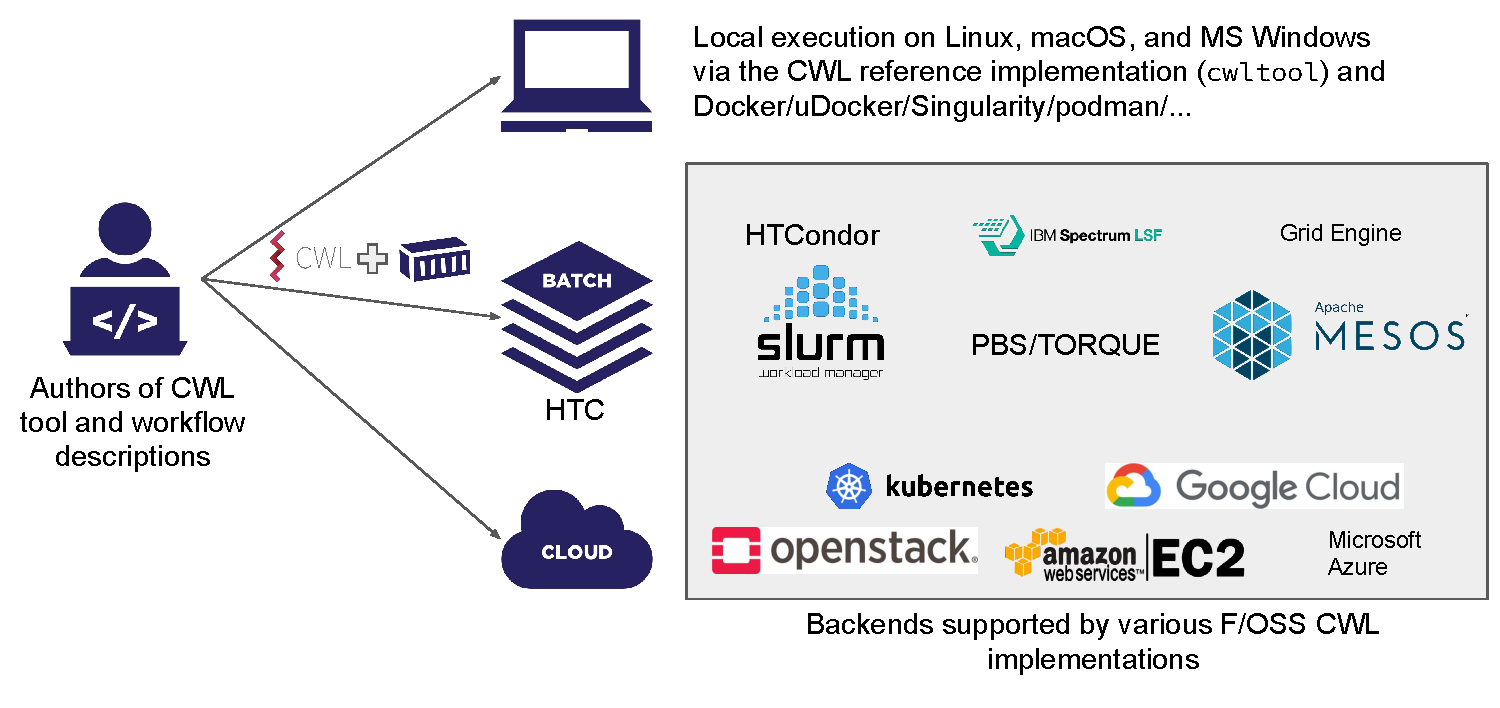
\includegraphics[width=0.8\textwidth]{methods_included/figure3}
  \vspace*{-0.5cm}
  %\includegraphics[width=1.0\textwidth]{figure2}
  %\vspace*{-1cm}
  \caption{\emph{Example of CWL portability.} The same workflow description runs on the scientist's own laptop or single machine, on any batch production-environment, and on any common public or private cloud. The CWL standards enable execution-portability by being explicit about data locations and execution models.} 
  \label{fig:portability}
\end{figure*}

\textbf{The explicit runtime model enables portability}, by being explicit about data locations. As Figure~\ref{fig:portability} indicates, this enables execution of CWL workflows on diverse environments as provided by various implementations of the CWL standards: the local environment of the author-scientist (e.g., a single desktop computer, laptop, or workstation), a remote batch production-environment~(e.g., a cluster, an entire datacenter, or even a global multi-datacenter infrastructure), and an on-demand cloud environment.

{The CWL standards explicitly support the use of \textit{software container} technologies, such as Docker and Singularity, to enable portability of the underlying analysis tools. Figure~\ref{fig:syntax}B, item 2, illustrates the process of pulling a Docker container-image from the \url{Quay.io} registry; then, the workflow engine automates the mounting of files and folders within the container. The container included in the figure has been developed by a trusted author and is commonly used in the bioinformatics field with an expectation its results are reproducible. Indeed, the use of containers can be seen as a confirmation that a tool’s execution is reproducible, when using only its explicitly declared runtime-environment. Similarly, when \textit{distributed execution} is desired, no changes to the CWL tool-description are needed: because the file or directory inputs are already explicitly defined in the CWL description, the (distributed) workflow runner can handle (without additional configuration) both job placement and data routing between compute nodes.

Via these two features (special handling of data paths; the optional but recommended use of software containers), the CWL standards enables portability (execution “without change”). Although various factors not controllable by software container technology can affect portability (e.g., variation in the underlying operating system kernel; variation in processor results), in practice the exact same software container and data inputs lead to portability without further adjustment from the user.

To support features that are \textit{not} in the CWL standards, the CWL standards define \textit{extension points} that permit (namespaced) vendor-specific features in explicitly defined ways. If these extensions do not fundamentally change how the tool should operate, then they are added to the \textit{hints} list and other CWL compatible engines can ignore them. However, if the extension is required to properly run the tool being described, e.g., due to the need for some specialized hardware, then the extension is listed under \textit{requirements} and CWL compatible engines can recognize and explicitly declare their inability to execute that CWL description.

The \textbf{CWL Workflow Description Standard}\footnote{\url{https://w3id.org/cwl/v1.2/Workflow.html}} builds upon the CWL Command Line Tool Standard: it has the same YAML- or JSON-style syntax, with explicit workflow level inputs, outputs, and documentation~(see Figure~\ref{fig:syntax}C). The workflow descriptions consists of a list of \textit{steps}, comprised of CWL CommandLineTools or CWL sub-workflows, each re-exposing their tool's required \textit{inputs}. Inputs for each step are connected by referencing the name of either the common \textit{workflow inputs} or particular outputs of other steps. The \textit{workflow outputs} expose selected outputs from workflow steps, making explicit which intermediate step outputs will be returned from the workflow. All connections include identifiers, which CWL document authors are encouraged to name meaningfully, e.g., \texttt{reference\_genome} instead of \texttt{input7}.

CWL workflows form explicit \textit{data flows}, as required for the particular computational analysis. The connectivity between steps defines the partial execution order. Parallel execution of steps is permitted and encouraged whenever multiple steps have all of their inputs satisfied, e.g., in Figure~\ref{fig:sample_workflow}, \texttt{find\_16S\_matches} and \texttt{find\_S5\_matches} are at the same data dependency level and can execute concurrently or sequentially in any order. Additionally, a \textit{scatter} construct allows the repeated execution of a CWL step (perhaps overlapping in time, depending on the resources available) where most of the inputs are the same except for one or more inputs that vary. This is done without requiring the modification of the underlying tool description. Starting with CWL version 1.2, workflows can also conditionally \textit{skip execution} of a (tool or workflow) step, based upon a specified intermediate input or custom boolean evaluation. Combining these features allows for a flexible \textit{branch} mechanism that allows workflow engines to calculate data dependencies before the workflow starts, and thus retains the predictability of the data flow paradigm.

In contrast to hard-coded approaches that rely on implicit file-paths particular for each workflow, CWL workflows are more \textit{flexible}, \textit{reusable}, and \textit{portable} (which enables scalability). The use in the CWL standards of explicit runtime environments, combined with explicit inputs/outputs to form the data flow, enables step reordering and explicit handling of iterations. The same features enable \textit{scalable} remote execution and, more generally, flexible use of runtime environments. Moreover, individual tool definitions from multiple workflows can be reused in any new workflow. 

CWL workflow descriptions are also \textit{future-proof}. Forward compatibility of CWL documents is guaranteed, as each CWL document declares which version of the standards it was written for and minor versions do not alter the required features of the major version. A stand-alone upgrader\footnote{\url{https://pypi.org/project/cwl-upgrader/}} can automatically upgrade CWL documents from one version to the next, and many CWL-aware platforms will internally update user-submitted documents at runtime.


\subsection{Execution of workflows in CWL format} \label{sec:execution}
CWL is a set of standards, not a particular software product to install, purchase, or rent. The CWL standards need to be implemented to be useful; a list of some implementations of the CWL standards is in Table \ref{tab:runners}. Workflow/tool runners that claim compliance with the CWL standards are allowed significant flexibility in how and where they execute a user's CWL documents as long as they fulfill the requirements written in those documents. For example, they are allowed (and encouraged) to distribute execution of a workflow across all available computers that can fulfill the resource requirements specified by the user. Aspects of execution not defined by the CWL standards include (web) APIs for workflow execution and real-time monitoring.

For example details about when a step should be considered ready for execution are available in §4 of CWL Workflow Description standard\footnote{\url{https://w3id.org/cwl/v1.2/Workflow.html\#Workflow}} but once all the inputs are available the exact timing is up to the workflow engine itself. 

Step execution may result in a temporary or permanent failure, as defined in §4 of CWL Workflow Description standard\footnote{\url{https://w3id.org/cwl/v1.2/Workflow.html\#Workflow_success_and_failure}}. It is up to the workflow engine to control any automatic attempts to recover from failures, e.g., to re-execute a Workflow step. Most workflow engines that implement the CWL standards offer the feature of attempting a number of re-executions, as set by the user, before reporting permanent failure.

The CWL community has developed the following optimizations without requiring that users re-write their workflows to benefit:
\begin{enumerate}
\item Automatic streaming of data inputs and outputs instead of waiting for all the data to be downloaded or uploaded (where those data inputs or outputs are marked with ``streamable: true'')
\item Workflow step placement based upon data location~\cite{jiang_tr-19-01_2019}, resource needs, and/or cost of data transfer~\cite{jiang_pivot_2019}
\item The re-use of the results from previously computed steps, even from a different workflow, as long as the inputs are identical. This can be controlled by the user via the ``WorkReuse'' directive\footnote{\url{https://w3id.org/cwl/v1.2/Workflow.html\#WorkReuse}}.
\end{enumerate}

Real world usage at scale: routinely CWL users and vendors report that they analyze 5000 whole genome sequences in a single workflow execution; one customer of a commercial vendor reported a successful run of a workflow that contained an 8,000-wide step; the entire workflow had 25,000 container executions. By design, the CWL standards do not impose any technical limitations to the size of files processed or to the number of tasks run in parallel. The major scalability bottlenecks are hardware-related --- not having enough machines with enough memory, compute or disk space to process more and more data at a larger scale. As these boundaries move in the future with technological advances, the CWL standards should be able to keep up and not be a cause of limitations.

\subsection{When is CWL not useful?} \label{sec:limitations}
The CWL standards were designed for a particular style of command-line tool based data analysis. Therefore, the following situations are out of scope and not appropriate (or possible) to describe using CWL syntax:

\begin{enumerate}
\item Safe interaction with stateful (web) services
\item Real-time communication between workflow steps
\item Interactions with command line tools beside 1) constructing the command line and making available file inputs (both user provided and synthesized from other inputs just prior to execution) and 2) consuming the output of the tool once its execution is finished, in the form of files created/changed, the POSIX standard output and error streams, and the POSIX exit code of the tool
\item Advanced control-flow techniques beyond conditional steps
\item Runtime workflow graph manipulations: dynamically adding or removing new steps during workflow execution, beyond any predefined conditional step execution tests that are in the original workflow description
\item Workflows that contain cycles: ``repeat this step or sub-workflow a specific number of times'' or ``repeat this step or sub-workflow until a condition is met.''\footnote{Supporting cycles/loops as an optional feature has been suggested for a future version of the CWL standards, but it has yet to be put forth as a formal proposal with a prototype implementation. As a work around, one can launch a CWL workflow from within a workflow system that does support cycles, as documented in the eWaterCycle case study with Cylc~\cite{oliver_workflow_2019}.}
\item Workflows that need particular steps run at or during a specific day/time-frame
\end{enumerate}

\section{Open-Source, Open Standards, Open~Community} \label{sec:open}

Given the numerous and diverse set of potential users, implementers, and other stakeholders, we posit that a project like CWL requires the combined development of code, standards, and community. Indeed, these requirements were part of the foundational design principles for CWL~(Section~\ref{sec:open:principles}); in the long run, these have fostered free and open source software~(Sidebar~B, in Section~\ref{sec:sidebar:b}), and a vibrant and active ecosystem~(Section~\ref{sec:open:ecosystem}). 

\subsection{The CWL Principles} \label{sec:open:principles}

The CWL project is based on a set of five principles:

\textbf{Principle 1}: The core of the project is the community of people who care about its goals.

\textbf{Principle 2}: To achieve the best possible results, there should be few, if any, barriers to participation. Specifically, to attract people with diverse experiences and perspectives, there must be no cost to participate.

\textbf{Principle 3}: To enable the best outcomes, project outputs should be used as people see fit. Thus, the standards themselves must be licensed for reuse, with no acquisition price.

\textbf{Principle 4}: The project must not favor any one company or group over another, but neither should it try to be all things to all people. The community decides.

\textbf{Principle 5}: The concepts and ideas must be tested frequently: tested and functional code is the beginning of evaluating a proposal, not the end.

In time, the CWL project-members learned that this approach is a superset of the OpenStand Principles\footnote{\url{https://open-stand.org/about-us/principles/}}, a joint ``Modern Paradigm for Standards'' promoted by the IAB, IEEE, IETF, Internet Society, and W3C. The CWL project's additions to the OpenStand Principles are: (1) to keep participation free of cost, and (2) the explicit choice of the Apache 2.0 license for all its text, conformance tests, and reference implementations.

\textbf{Necessary and sufficient}: All these principles have proven to be essential for the CWL project. For example, the free cost and open source license~(Principles~2 and~3) has enabled many implementations of the CWL standards, several of which re-use different parts of the reference implementation of the CWL standards (\textit{reference runner}). Being community-first~(Principle 1) has led to several projects from participants that are outside the CWL standards themselves; the most important contributions have made their way back into the project~(Principle~4).

As part of Principle 5, contributors to the CWL project have developed a suite of conformance tests for each version of the CWL standards. These publicly available tests were critical to the CWL project's success: they helped assess the reference implementation of the CWL standards themselves; they provided concrete examples to early adopters; and they enabled the developers and users of production implementations of the CWL standards to confirm their correctness.

\subsection{Sidebar B: The CWL project and Free/Open Source Software (F/OSS)}\label{sec:sidebar:b}

\subsubsection{Free and Open Source implementations of the CWL standards}\footnote{Snapshot of \url{https://www.commonwl.org/implementations/}}

By 2021, the CWL standards have gained much traction and are currently widely supported in practice. In addition to the implementations in Table \ref{tab:runners}, Galaxy~\cite{afgan_galaxy_2018}\footnote{\url{https://github.com/common-workflow-language/galaxy/pull/47}} and Pegasus~\cite{deelman_pegasus_2015}\footnote{\url{https://pegasus.isi.edu/documentation/manpages/pegasus-cwl-converter.html}} have in-development support for the CWL standards as well.

Wide adoption benefits from our principles: The CWL standards include conformance tests, but the CWL community does not yet test or certify implementations of the CWL standards, or specific technology stacks. Instead, the authors and service provides of workflow runners and workflow management systems self-certify support for the CWL standards, based on a particular technology configuration they deploy and maintain.

\begin{table}
  \caption{Selected F/OSS workflow runners and platforms that implement the CWL standards.}
  \label{tab:runners}
    \begin{tabular}{ll}
      \toprule
      Implementation & Platform support\\
      \midrule
      \href{https://pypi.org/project/cwltool}{cwltool} & Linux, macOS, Windows (via WSL 2) \\
      & local execution only\\
      \href{https://arvados.org}{Arvados} & in the cloud on AWS, Azure and GCP, \\
      & on premise \& hybrid clusters using Slurm \\
      & or LSF\\
      \href{https://pypi.org/project/toil-cwl-runner}{Toil}\cite{vivian_toil_2017} & AWS, Azure, GCP, Grid Engine, HTCondor, \\
      & LSF, Mesos, OpenStack, Slurm, PBS/Torque\\
      & also local execution on Linux, macOS, \\
      & MS Windows (via WSL 2)\\
      \href{https://pypi.org/project/cwl-airflow}{CWL-Airflow}\cite{kotliar_cwl-airflow_2019} & Local execution on Linux, OS X\\
      & or via dedicated Airflow enabled cluster.\\
      \href{https://streamflow.di.unito.it/}{StreamFlow}\cite{colonnelli_streamflow_2020} & Kubernetes, HPC with Singularity \\
      & (PBS, Slurm), Occam, multi-node SSH, \\
      & local-only (Docker, Singularity)\\
      \href{https://docs.reana.io/}{REANA} & Kubernetes
      %\bottomrule
\end{tabular}
\end{table}

\subsubsection{F/OSS tools and libraries for working with CWL format documents}\footnote{Summarized from \url{https://www.commonwl.org/tools/}}\label{sec:sidebar:b:workwith}

CWL plugins for text/code editors exist for Atom, vim, emacs, Visual Studio Code, IntelliJ, gedit, and any text editor that support the ``language server protocol'' \footnote{\url{https://microsoft.github.io/language-server-protocol/}} standard.

There are tools to generate CWL syntax from Python (via argparse/click or via functions), ACD{\footnote{``Ajax Command Definitions'' as produced by the EMBOSS tools: \url{http://emboss.sourceforge.net/developers/acd/}}, CTD\footnote{XML-based ``Common Tool Descriptors''~\cite{de_la_garza_desktop_2016} originating in the OpenMS project: \url{https://github.com/WorkflowConversion/CTDSchema}}, and annotations in IPython Jupyter Notebooks. Libraries to generate and/or read CWL documents exist in many languages: Python, Java, R, Go, Scala, Javascript, Typescript, and C++.

\subsection{The CWL Ecosystem}\label{sec:open:ecosystem}

Beyond the ratified initial and updated CWL standards released over the last six years, the CWL community has developed many \textit{tools, software libraries, connected specifications}, and has shared CWL descriptions for popular tools. For example, there are software development kits for both Python\footnote{\url{https://pypi.org/project/cwl-utils/}} and Java\footnote{\url{https://github.com/common-workflow-lab/cwljava}} that are generated automatically from the CWL schema; this allows programmers to load, modify, and save CWL documents using an object oriented model that has direct correspondence to the CWL standards themselves. CWL SDKs for other languages are possible by extending the code generation routines\footnote{See the \texttt{*codegen*.py} files in \url{https://pypi.org/project/schema-salad/7.1.20210316164414/}}. (See Sidebar B in Section~\ref{sec:sidebar:b:workwith} for practical details.)

The CWL standards support well the acute \textit{need to reuse} (and, correspondingly, \textit{to share}) information on workflow execution, and on authoring and provenance. The CWLProv\footnote{\url{https://w3id.org/cwl/prov/}} prototype was created to show how existing standards~\cite{belhajjame_using_2015,kunze_bagit_2018,missier_w3c_2013} can be combined to represent the provenance of a specific execution of a CWL workflow~\cite{khan_sharing_2019}. Although, to-date, CWLProv has only been implemented in the CWL reference runner, interest is high in additional implementation and further development.

\section{Conclusion}\label{sec:conclusion}

The problem of standardizing computational reuse is only increasing in prominence and impact. Addressing this problem, various domains in science, engineering, and commerce have already started to migrate to workflows, but efforts focusing on the portability and even definition of workflows remain scattered. In this work we raise awareness to this problem and propose a community-driven solution.

The Common Workflow Language (CWL) is a family of standards for the description of command line tools and of workflows made from these tools. It includes many features developed in collaboration with the community: support for software containers, resource requirements, workflow-level conditional branching, etc. Built on a foundation of five guiding principles, the CWL project delivers open standards, open-source code, and an open community.

For the past six years, the community around CWL has developed organically. 
Organizations looking to write, use, or fund data analysis workflows based upon command-line tools should adopt or even require the CWL standards, because the CWL standards offer a common yet reduced set of capabilities that are both used in practice and implemented in many popular workflow systems. CWL is further valuable because it is supported by a large-scale community, diverse fields have already adopted it, and its adoption is rapidly growing.
Specifically,
\begin{enumerate}
\item By using a reduced set of capabilities, the CWL standards limit the complexity encountered by users when they start to use it, and by operators when they have to implement it. (Feedback from the community indicates these are appreciated.)
\item By using declarative syntax, CWL allows users to specify workflows even if they do not know exactly where the workflows would (later) run. 
\item The CWL project is governed in the public interest and produces freely available open standards. The CWL project itself is not a specific workflow management system, workflow runner, or vendor. This allows potential users, operators, and vendors, to avoid lock-in and be more flexible in the future.
\item By offering standards, the CWL project distinguishes itself especially for the complex interactions that appear in scientific and engineering collaborations. These interactions include defining workflows from many different tools (or steps), sharing workflows, long-term archiving, fulfilling requirements of regulators (e.g., US FDA), making workflow executions auditable and reproducible. (This is particularly useful in cooperative environments, where groups that compete with each other need to collaborate, or in scientific papers where the paper results can be reused very efficiently if the analysis is described in a CWL workflow with publicly available software containers for all steps.)
\item The CWL standards are already implemented, adopted, and used; with many production-grade implementations available as open source and with zero-cost. Thus, the different communities of users of the CWL standards already offer numerous workflow and tool descriptions. (This is akin to how the Python ecosystem of shared libraries, code, and recipes is already helpful.) 
\end{enumerate}

To conclude: this is a call for others to embrace workflow thinking and join the CWL community in creating and sharing portable and complete workflow descriptions. With the CWL standards, the methods are included and ready to (re)use}!

The CWL project is immensely grateful to the following self-identified CWL Community members and their contributions to the project:
\contributor{https://orcid.org/0000-0002-2703-8936}{Miguel d'Arcangues Boland}{Software, Bug Reports, Maintenance},
\contributor{}{Alain Domissy}{Conceptualization, Answering Questions, Tools},
\contributor{}{Andrey Kislyuk}{Software, Bug Reports},
\contributor{https://orcid.org/0000-0001-7811-8613}{Brandi Davis-Dusenbery}{Conceptualization, Funding acquisition, Investigation, Project Administration, Resources, Supervision, Business
Development, Event Organizing, Talks},
\contributor{https://orcid.org/0000-0001-9795-7981}{Niels Drost}{Funding Acquisition, Blogposts, Event Organizing, Tutorials, Talks},
\contributor{https://orcid.org/0000-0001-8626-2148}{Robert Finn}{Data acquisition, Funding acquisition, Investigation, Resources, Supervision},
\contributor{https://orcid.org/0000-0001-9292-1533}{Michael Franklin}{Software, Bug Reports, Documentation, Event Organizing, Maintenance, Tools, Answering Questions, Talks},
\contributor{https://orcid.org/0000-0002-5843-4712}{Manabu Ishii}{Blogposts, Documentation, Examples, Event Organizing, Maintenance, Tools, Answering Questions, Translation, Tutorials, Talks},
\contributor{https://orcid.org/0000-0003-4115-3313}{Sinisa Ivkovic}{Software, Validation, Bug Reports, Tools},
\contributor{https://orcid.org/0000-0002-3468-0652}{Alexander Kanitz}{Software, Business Development, Tools, Talks},
\contributor{https://orcid.org/0000-0002-5044-4692}{Sehrish Kanwal}{Conceptualization, Formal Analysis, Investigation, Software, Validation, Bug Reports, Blogposts, Content, Event Organizing, Maintenance, Answering Questions, Tools, Tutorials, Talks, User Testing},
\contributor{https://orcid.org/0000-0001-9102-5681}{Andrey Kartashov}{Conceptualization, Software, Validation, Examples, Tools, Answering Questions},
\contributor{https://orcid.org/0000-0002-6337-3037}{Farah Khan}{Conceptualization, Formal Analysis, Funding Acquisition, Software},
\contributor{https://orcid.org/0000-0002-6486-3898}{Michael Kotliar}{Software, Validation, Bug Reports, Blogposts, Examples, Maintenance, Answering Questions, Reviewed Contributions, Tools, Talks, User Testing},
\contributor{https://orcid.org/0000-0003-1112-2284}{Folker Meyer}{Tools},
\contributor{https://orcid.org/0000-0002-6388-7353}{Rupert Nash}{Software, Bug Reports, Talks, Videos},
\contributor{https://orcid.org/0000-0003-3705-948X}{Maya Nedeljkovich}{Software, Validation, Visualization, Writing -\/- review \& editing, Bug Reports, Tools, Talks},
\contributor{https://orcid.org/0000-0003-3777-5945}{Tazro Ohta}{Formal Analysis, Funding Acquisition, Resources, Validation, Bug Reports, Blogposts, Content, Documentation, Examples, Event Organizing, Answering Questions, Tools, Translation, Tutorials, Talks, User Testing},
\contributor{https://orcid.org/0000-0002-8021-9162}{Pjotr Prins}{Blogposts, Packaging, Bug Reports},
\contributor{https://orcid.org/0000-0001-9279-9910}{Manvendra Singh}{Software, Blogposts, Packaging, Tools, Reviewed Contributions},
\contributor{https://orcid.org/0000-0002-0959-4429}{Andrey Tovchigrechko}{Conceptualization, Software, Bug Reports},
\contributor{https://orcid.org/0000-0003-3156-2105}{Alan Williams}{Investigation},
\contributor{https://orcid.org/0000-0002-6130-1021}{Denis Yuen}{Software, Bug Reports, Documentation, Tools},
\contributor{https://orcid.org/0000-0002-0415-9655}{Alexander (Sasha) Wait Zaranek}{Conceptualization, Funding Acquisition},
\contributor{https://orcid.org/0000-0003-4716-9121}{Sarah Wait Zaranek}{Conceptualization, Funding Acquisition, Project Administration, Resources, Software, Accessibility, Bug Reports, Business Development, Content, Examples, Event Organizing, Answering Questions, Tutorials, Talks}.

The contributions to the CWL project by the authors of this paper are:
\contributor{https://orcid.org/0000-0002-2961-9670}{Michael R. Crusoe}{Conceptualization, Funding Acquisition, Investigation, Project Administration, Resources, Software, Supervision, Validation, Writing --- original draft, Bug Reports, Business Development, Content, Documentation, Examples, Event Organizing, Maintenance, Packaging, Answering Questions, Reviewing Contributions, Tutorials, Talks},
\contributor{https://orcid.org/0000-0002-2779-7174}{Sanne Abeln}{Writing --- original draft, and review \& editing, Conceptualization, Supervision, Funding acquisition},
\contributor{https://orcid.org/0000-0001-8030-9398}{Alexandru Iosup}{Writing --- original draft, and review, editing, Conceptualization, Supervision, Funding acquisition},
\contributor{https://orcid.org/0000-0003-3566-7705}{Peter Amstutz}{Conceptualization, Formal Analysis, Funding Acquisition, Methodology, Project Administration, Resources, Software, Supervision, Validation, Visualization, Bug Reports, Business Development, Content, Documentation, Examples, Event Organizing, Maintenance, Packaging, Answering Questions, Reviewed Contributions, Security, Tools, Tutorials, Talks},
\contributor{https://orcid.org/0000-0001-8316-4067}{Nebojša Tijanić}{Conceptualization, Software},
\contributor{https://orcid.org/0000-0002-7552-1009}{Hervé Ménager}{Conceptualization, Funding Acquisition, Investigation, Methodology, Project Administration, Resources, Software, Supervision, Bug Reports, Business Development, Examples, Event Organizing, Maintenance, Tools, Tutorials, Talks},
\contributor{https://orcid.org/0000-0001-9842-9718}{Stian Soiland-Reyes}{Conceptualization, Funding Acquisition, Investigation, Project Administration, Resources, Software, Supervision, Validation, User Testing, Writing – review and editing, Bug Reports, Blogposts, Business Development, Content, Documentation, Examples, Event Organizing, Packaging, Tools, Answering Questions, Reviewed Contributions, Security, Tutorials, Talks, Videos},
\contributor{https://orcid.org/0000-0003-1550-1716}{Bogdan Gavrilovic}{Conceptualization, Software, Validation, Bug Reports, Blogposts, Maintenance, Tools, Answering Questions, Reviewed Contributions, User Testing},
\contributor{https://orcid.org/0000-0003-1219-2137}{Carole A. Goble}{Conceptualization, Funding Acquisition, Resources, Supervision, Audio, Business Development, Content, Examples, Event Organizing, Tools, Talks, Videos}.

\def\grantsponsor#1#2#3{#2}                                                     
\newcommand\grantnum[3][]{#3%                                                   
  \def\@tempa{#1}\ifx\@tempa\@empty\else\space(\url{#1})\fi}

Funding acknowledgements: \grantsponsor{EU}{European Commission}{https://ec.europa.eu/programmes/horizon2020/} grants  
BioExcel-2 (SSR)  \small\grantnum[https://cordis.europa.eu/project/id/823830]{EU}{H2020-INFRAEDI-02-2018 823830}\normalsize,
BioExcel (SSR) \small\grantnum[https://cordis.europa.eu/project/id/675728]{EU}{H2020-EINFRA-2015-1 675728}\normalsize,
EOSC-Life (SSR) \small\grantnum[https://cordis.europa.eu/project/id/824087]{EU}{H2020-INFRAEOSC-2018-2 824087}\normalsize,
EOSCPilot (MRC) \small\grantnum[https://cordis.europa.eu/project/id/739563]{EU}{H2020-INFRADEV-2016-2 739563}\normalsize,
IBISBA 1.0 (SSR) \small\grantnum[https://cordis.europa.eu/project/id/730976]{EU}{H2020-INFRAIA-2017-1-two-stage 730976}\normalsize,
ELIXIR-EXCELERATE (SSR, HM) \small\grantnum[https://cordis.europa.eu/project/id/676559]{EU}{H2020-INFRADEV-1-2015-1 676559}\normalsize,
ASTERICS (MRC) \small\grantnum[https://cordis.europa.eu/project/id/653477]{EU}{INFRADEV-4-2014-2015 653477}\normalsize. \grantsponsor{ELIXIR}{ELIXIR}, the research infrastructure for life-science data, Interoperability Platform Implementation Study (MRC). \small\grantnum[https://elixir-europe.org/about-us/commissioned-services/cwl-2018]{ELIXIR}{2018-CWL}\normalsize.  Various universities have also co-sponsored this project; we thank Vrije Universiteit of Amsterdam, the Netherlands, where the first three authors have their primary affiliation.


\chapter{CWL Deep Dive}
\label{cwl-deep-dive}


\dropcap{C}ommon Workflow Language is ...

In \cite{crusoe-methods-2022} we described how the CWL community came to be, the community's goals and ways of working.

In this chapter I will take a deeper dive into the technical decisions made by the CWL Community (of which I'm a co-founder, later CWL Community Engineer and since 2018 the CWL Project Leader).

%Target: IEEE Transactions on Parallel and Distributed Systems (TPDS)
%Audience: future students to explain my work and way of working
%FOCUS ON: 
%Design choices
%Implementation choices
%Practical use
%Lessons learned
%Comparison with state-of-the-art


%Sufficiency / necessity argument: high level comparison with alternatives/competitors
%Repeat qualitative analysis for other popular workflow languages (WDL, SnakeMake, Nextflow, Galaxy)
%sufficient --> has all features
%necessary --> first/only one to have _all_
%Column A1: core workflow patterns (almost all have it) ← evidence + expert interpretation
%A2: conformance test (few have it) ← evidence based
%A3: ... (community developed) ← argumentative
%A4: multiple independent implementations ← evidence based


% Need to explain each decision; for each: what were the alternatives and why weren’t they chosen?
% 
% Relationship with control-flow workflows (systems): (data-flow workflows go inside control-flow workflows, not the other way around)
% 
% Design choices
% 
% Build upon existing standards (POSIX, OCI, YAML, JSON-LD, RDF)
% Separation of concerns: <details needed>
% (often with accompanying Docker format software containers)
% Focus on the workflow author (IDE integrations, syntax choices, future plans)

\section{The Problem of Standardization}

A standard is the named communication of an existing agreement between a group to a larger context. Therefore prior to standardization that group has to come to an agreement and precisely define their shared understanding. Initially the group that became the CWL community looked at codifying an existing workflow and tool description language (specifically Galaxy) as the basis for a standardized workflow language. After a deeper examination it was found by Galaxy core developers that due to Galaxy’s many years of organic growth and an early choice about how to enable templating and advanced command line construction\footnote{Galaxy’s tool description format allows for Python expressions. However the Galaxy workflow engine is written in Python and due to other technical reasons this meant that tool description authors had access to all Galaxy internals from their tool descriptions. Therefore, for other systems to implement the Galaxy tool description format they would need the entire Galaxy Python codebase (or an implementation of it) available as well.} made it unsuitable to codify the Galaxy tool description language directly into a standard. Therefore the decision was made to make a new workflow and tool description language, building on the lessons learned from the multitude of workflow languages and systems before.

Making a new workflow language, even working from the perspective of many decades of collective experience, is not a small undertaking. Add to that the creation of a precise specification, conformance tests, and many implementations and one sees why standardization and the necessary work that both precedes that succeeds standardization needs to be weighed against the potential and likely benefits.

\section{An Idealized Workflow Language}
%<AI->MC: Explain what kinds of issues such a language would address, preferably with brief examples. Then, you can derive naturally the goals. // could go in the Introduction (goals for the next decade, but here we take one step toward standardization)>

Workflow issues circa 2014: 
1. tool/workflow descriptions that depend on engine/platform implementation details are non-portable
2. lack of standard or shared language meant that tool authors or 3rd parties describing tools have to support each workflow system separately. For complex command-line tools, or ones that changed quickly, this maintenance burden was substantial
3. some workflow approaches did not scale well with larger sets of data or increasing complexity of the workflow (common with Make-like systems that encode step names, replica and sample IDs and other organizational details in the filenames assigned to data)
4. Most "in house" workflow systems bake in local computing facility details (names of servers, specific filesystem mount paths) that prevent anyone using even the same code at another institute without (perhaps significant) modification.
5. Existing standards in the workflow space were not relevant to most scientific workflows; instead focused on control-flow and business process workflows.

\subsection{Goals}
Standardized functional portable description of command-line tools and dataflow workflows made up of them
(these descriptions are able to be complete enough to execute)
There should not be implementation or vendor specific details in the specification.
Improve communication and understanding between workflow author and users labels / human friendly identifiers / subworkflows
That data and inputs are explicit and they have identifiers
All the hallmarks of a good workflow system (ASAP) are supported directly or indirectly
Being a good player in the ecosystem by supporting the 17 FAIR Principles where possible. (See section 5 for more details).

\subsection{Non-Goals}
Supporting every theorized workflow construct ; the “Common” in CWL is about targeting the features that are both commonly used by workflow authors and commonly implemented by workflow engines.
(web) service orchestration / interaction with external stateful systems 
Why not? they have state, can go away, not idempotent, not reproducible. (The Taverna experience) Services are not bad, but they need to give the users the workflow and references to the reference data used
Neither business process management nor other control-flow approaches
(no stopping for external decision making, which is not reproducible). CWL tools/workflows could be called from a business process management.
not a strict guarantee of reproducibility

\section{The Design of CWL}
\subsection{Overview}
Two sets of features for the 2 standards
% one visual
\subsection{Design Choices}
\subsubsection{Unit of compute: POSIX command line tools.}

* Supports Goal \#1

* In bioinformatics, command line tools vastly outnumber services and GUIs
* The POSIX application interface is well understood and widely used
* The model in summary: inputs are a list of strings, outputs are written to the filesystem, STDOUT, and STDERR. Assume that exit code of not 0 is an error, this is customizable. CWL v1.2 allows capturing the exit code for further use.
* Services were not chosen as they are too fragile and immature compared to POSIX; experience with Taverna and other systems showed that many advanced concepts are needed to cope. Services are rarely 1st class components of workflow systems, so not a good candidate for a “common” language.

\subsubsection{connection between compute and data into a full workflow (the dataflow model)}
Necessary to have enough information to support Goal \#1 and \#4
We must document all connections between tasks, even those that a user might not be aware of
This enables portability regardless of the execution environment being  distributed or having a shared filesystem. It also enable better provenance tracking
CWL’s object model does not use strings to track file or directory inputs and outputs, instead using a simple dictionary of properties (“class: File” and “class: Directory”). These objects do not assign a path to a File or Directory until just prior to tool execution. Instead Files and Directory have a “location” identifier, and the name of the File or Directory is also stored separately, allowing the location IRI to be meaningful to the workflow engine.
Alternatives:

\subsubsection{file streaming is supported but not required}
A common optimization pattern in hand written workflows
If marked as such, CWL allows File inputs/outputs to be implemented using a named pipe, a.k.a “|”
This allows workflow systems to speed up execution by streaming data into/out-of object stores or directly between tasks
All “type: stdin”, “type: stdout”, and “type: stderr” Inputs/Output have this potential without further specification by the user. Otherwise they can add `streamable: true’ to any Input/Output of `type: File` or `type: File[]`
This was a simple thing to add to the CWL specification, so not adding it was not seriously considered. However, exploitation of this feature has only been done by one engine: toil-cwl-runner.

\subsubsection{no tool to tool IP based communication}
Would violate anti-goal \#1
Ensuring a network path may be non-trivial or not allowed in some workflow execution systems ; implies co-scheduling, which is not very common
Lots of costs to implement this and often not needed, so we kept it out of CWL very early on
CWL has no construct to specify parallel co-scheduling nor port coordination
There are many frameworks and libraries for service orchestration, users are encouraged to use them if that is their need

\subsubsection{syntax choices (balance between readability and using off the shelf libraries for parsing)}
While CWL is regular enough for automated conversion to/from, or programmatic assembly, we knew that users would still be writing/editing by hand (especially during the early phases of adoption) (Goal \#3)
When a design decision came down to an option being more convenient for users versus implementers, we often chose the users. Planned revisions to the standards will include even more user focused design patterns.
Many users of CWL will be causal and infrequently interacting with CWL. By favoring users we make the language more attractive and increase the likelihood of adoption
Examples: map<> syntax simplification; YAML;
JSON? Can’t have comments ; new DSL? Harder to implement, not necessarily more readable for users. XML? gross.

\subsubsection{Review of workflow constructs supported}
(explain why and cross-reference the workflow patterns repository) See \url{https://github.com/common-workflow-library/cwl-patterns/tree/master/workflow_patterns_initiative}

\subsubsection{Optional parts}

To support a diverse ecosystem (Goal \#3). Some workflow engines may not want to / be able to implement all of the CWL syntax
What:
V1.0+: InlineJavascriptRequirement, SchemaDefRequirement, LoadListingRequirement, DockerRequirement, SoftwareRequirement, InitialWorkDirRequirement, EnvVarRequirement, ShellCommandRequirement, ResourceRequirement
V1.1+: WorkReuse, NetworkAccess, InplaceUpdateRequirement, ToolTimeLimit
V1.2+: (abstract) Operation processes (non-runnable, useful for provenance reporting from non-CWL systems), conditional execution of steps using `WorkflowStep.when`

One can use/implement the CWL CommandLineTool standard separate from the entire Workflow standard, if desired
This allows engines and other CWL consumers/produces to make progressively more useful tools while being able to communicate clearly what they support to users (and to fail quickly if given a document they can’t fully execute)
All of these features must be listed by the author of a CWL document, if used, except for conditional workflow steps in CWL v1.2+. Features mentioned under the “hints” section are allowed to be ignored by consumers of the document if they don’t (yet) support them. Features mentioned under “requirements” must be supported, and if they are not available then consumers of the document should fail early and inform the user why.
Feature detection by syntax (instead of these explicit feature flags) was considered and may be implemented in CWL 2.0 to simplify the syntax for the description author.

\subsubsection{Linked data and external ontologies}

Don’t reinvent the wheel, Supports Goals 2,3, 4
File formats are complicated and often very domain specific. Likewise metadata models for workflows and tools
The external ontologies are governed and maintained by experts and contributors, each on their own cadence separate from the CWL standards cadence. Therefore they can be improved/extended without waiting for a new release of CWL
The EDAM ontology is a popular source of identifiers for bioinformatic file formats and it models the relationship between them along with many other useful aspects. For CommandLineTool and Workflow metadata, it is recommended (but not mandatory) to use the schema.org ontology.
Bundling specific baseline versions of some of these ontologies in CWL as a shortcut for users has been considered and might appear in a future version of the standards.
\url{https://www.commonwl.org/v1.1/Workflow.html#Extensions_and_metadata}

\subsubsection{software containers}
Optional, but recommended! Docker format, engine agnostic (Singularity, podman, apptainer, docker, etc..)
Software installation is said to be the hardest problem in bioinformatics and many other research fields
Therefore CWL supports the specification of an recommended (or required) Docker format software container as part of the CommandLineTool specification
This helps (but does not guarantee) reproducibility
Under “DockerRequirement”, tool description authors can specify one of the following: the name of a docker/OCI format image from a registry (defaulting to hub.docker.com but others are allowed) ; a URL to a docker/OCI format image ; an in-place “Dockerfile” format recipe for Docker/OCI format image construction
When CWL began, the Open Container Initiative was in its infancy. It is planned that future versions of the CWL standards will refer to the OCI standards more directly. The Docker engine is not a requirement for fulfilling the “DockerRequirement”, any engine that support the Docker image format (directly or indirectly) is a valid choice by a CWL compliant engine; this includes Singularity, udocker,
\subsubsection{Mechanism for extensions}
Allows and encourages vendors/users to develop/use well marked extensions to the CWL standards
As CWL aims to support features that are “common”ly used by people and “common”ly implemented by engines, it shouldn’t get in the way of those who want to build upon it
Now that CWL is more stable and more widely deployed, getting vendors to experiment with new features and then learning from their experiences provides a better model for stable enhancement
All extensions must be a URL (often abbreviated using the \$namespace feature) and preferably resolve to a web page with more information about the extension. Several features that exist in post v1.0 version of CWL came from vendor extensions: TimeLimit, WorkReuse (previously \url{http://arvados.org/cwl#ReuseRequirement} ), NetworkAccess, InplaceUpdateReqirement, LoadListingRequirement. Like the optional features of CWL, they can be specified under the “hints” section if they can be safely ignored, or under “requirements” if they are necessary for proper execution.
The alternative would be secret extensions/changes that would be hard to detect prior to tool/workflow execution which would hamper reproducibility/ reusability.
\subsubsection{conformance tests}
Need to be able verify the behavior of the various CWL implementations (Goal \#2)
Conformance tests that target different features, their aspects, and combinations of the above along with specified correct output (or a flag that the provided input should result in an error). The tests are tagged with the names of optional features used, if any.
This provides assurances to users that their CWL documents will work in multiple environments, and helps engine authors make progress as they implement CWL features
Conformance tests are developed in conjunction with releases of the CWL standards. They are available under the Apache 2.0 license.
We wrote our own testing framework, but this is a prototype of a plugin to py.test that could be completed.
\subsubsection{Optional support for Javascript in very well defined circumstances}
As the CWL standards don’t aim to cover all possible needs especially when it comes to most extremely badly designed command line interfaces, a script language was chosen as an optional feature.
Users may provide values for certain fields in CWL using ECMAScript 5.1 (commonly known as Javascript). What objects are available to them in that context is tightly defined; no cross talk is allowed; and the order of parsing is explicit
This allows users to work around missing features without having to change the underlying program (which might not be possible or realistic). It also allows for cheap rearrangement of complex object trees without requiring scheduling a task and marshalling/unmarshalling data.
Users must specify that they need the `InlineJavascriptRequirement` under features. To distinguish the javascript from literal strings, it is wrapped in `${ }` for  ECMAScript function body style, or `$( )` for ECMAScript Expression style.
This has been a controversial feature. Many users (and the authors of the CWL standards themselves) would prefer to use Python, but the lack of secure Python VMs prevented this. Currently we are debating on how best to allow users to write CWL Expressions using newer versions of the ECMAScript standard while keeping backward compatibility. ECMAScript 5.1 is from 2011, but newer versions of ECMAScript are not completely backwards compatible with code that targets ECMAScript 5.1.
\subsubsection{Separation of concerns}
There are many audiences for a workflow or tool description and they can be divided into those who execute said description and those who write them.
In designing and refining the CWL standards, maintaining this separation of concerns cleanly was an important sub-goal.
This allows workflow/tool description authors to focus on their analysis and/or communication goals. Likewise it allows workflow engines to focus on optimizing the execution of these same descriptions.
The declarative syntax of CWL, the defined boundaries and expectations, and CWL being a standard and not a library or framework that must be included all give freedom to workflow engines authors to optimize as best they can. It even encourages “vertical engineering” where a workflow system is written, or heavily customized, for a specific technology stack as opposed to the traditional middleware “compatible with everything” approach that sacrifices speed and maintainability for flexibility.
From an engineering perspective, this separation of concerns is at the heart of CWL. Alternatives to this approach were not considered from the moment the founders decided to make a community standard.
\subsubsection{variety of execution models}
single-machine, cluster with a shared filesystem, and distributed
Researchers typically have access to a wide variety of computing capability, and their workflows should not need to be rewritten to be runnable elsewhere. (Portability from Goal \#1)
CWL’s object and execution model allow for execution on a single-machine, compute cluster with a shared filesystem, or distributed execution without a shared filesystem. None of this requires any changes to the tool nor workflow descriptions
Assumptions about paths, directory layouts, and other local details are quite common in hand written workflows. Once these workflow get very large (as they tend to do over time) this can be incredibly time consuming to abstract out. By building this into the CWL standards, everyone benefits without additional work.
As mentioned before, CWL does not represent the a file as a string, but instead as an object with properties, thus forcing the tool description author to be explicit about which inputs are files and which are not. Likewise, when forming a workflow by connecting the inputs and outputs of tools together, one does not do so by using file names or paths (like in a Makefile) but by using identifiers for particular outputs of particular steps which are often meaningful and concise.
5. alternatives not chosen, and why they weren't selected
\subsubsection{Differentiating between data paths and regular strings}
In the CWL object model, which can be queried and manipulated by CWL Parameter References and CWL Expressions, we distinguish between paths (to a file or a directory) and other strings.
While at the time of CommandLineTool execution a filesystem path will be synthesized, at all other times these objects are distinguished by a URI.
This URI might be meaningful to the engine directly (like an object store path) or it might be further transformed or queried internally.

\subsection{Syntax Examples of CWL}

\subsection{Support levels for optional features in CWL runners circa 2024}
% TODO: turn into a table
`toil-cwl-runner`: all of CWL v1.0-v1.2; `InplaceUpdateRequirement` is only supported when using a shared filesystem with the ``--bypass-file-store`` option.


\section{The CWL standards support the 17 FAIR Principles}
It is one of the goals of the CWL project to assist workflow engines/platforms and users in realizing the FAIR principles[3] while not imposing a burden for lack of perfection or completion. When considering the FAIR and CWL we examine not just the context of the workflow and tool descriptions, but also the context of creating, sharing, and executing these descriptions; and finally the context not narrowing the adherence of inbound data to the FAIR principles and increasing the adherence of the FAIR principles for the outbound data.

Rather than attempting to conduct a quantitative study, we focus here on qualitative analysis as the FAIR Principles are just that, principles, and not specific metrics. For specific data types there are specific community led FAIR metrics, but there are no universal FAIR metrics (nor should there be, as “FAIR is not a standard”[4]).
\subsection{To be Findable}
\subsubsection{F1. “(meta)data are assigned a globally unique and persistent identifier”}
In CWL, all items of type File, Directory, Workflow, and CommandLineTool have an identifier which can be “globally unique and eternally persistent” if available, or just locally meaningful. For example, the CWL reference implementation’s use of CWLProv generates random UUIDs for inputs, outputs, and intermediate values, but a workflow platform or service would use registered identifiers.
\subsubsection{F2. “data are described with rich metadata (defined by R1 below)”}
The CWL standards prescribe how Workflow and CommandLineTool descriptions can have arbitrary embedded metadata in a structured way. For generic metadata it is recommend to use the schema.org vocabulary. While community or domain specific metadata is also allowed and encouraged, the CWL standards do not prescribe any particular metadata standard, as that is a decision for specific groups to develop and evolve.
\subsubsection{F3. “metadata clearly and explicitly include the identifier of the data it describes”}
This is automatic for CWL documents, as the metadata is embedded in the data it describes.
\subsubsection{F4. “(meta)data are registered or indexed in a searchable resource”}
There are several registries of workflows, and one in particular (Workflow Hub) has chosen the CWL object model for their workflow metadata model, even for workflows not written using the CWL standards.
\subsection{To be Accessible}
\subsubsection{A1. “(meta)data are retrievable by their identifier using a standardized communications protocol”}
There is no official API for retrieving a CWL document via an identifier. Popular choices include HTTP and the “GA4GH Tool Registry API” (also known as GA4GH TRS). By retrieving a CWL description (data) one then has access to the embedded metadata (if any).

For retrieval of input data for the execution of a CWL workflow or tool, CWL allows for any URI scheme. HTTP(S) is available in all known CWL implementations (modulo local network policies) and many implementations support the relevant object storage protocols. GA4GH has an API specification (GA4GH DRS) for services that convert a data identifier into a platform (and perhaps region) specific URI. Using any of these protocols, their future versions, or entirely new protocols, requires no changes to the CWL standards as long as URI/IRIs are available.
\subsubsection{A1.1 “the protocol is open, free, and universally implementable”}
HTTP, GA4GH TRS, and GA4GH DRS all meet this requirement.
\subsubsection{A1.2 “the protocol allows for an authentication and authorization procedure, where necessary”}
HTTP meets this requirement. For GA4GH TRS they state that “GA4GH recommends the use of the OAuth 2.0 framework (RFC 6749) for authentication and authorization. It is also recommended that implementations of this standard implement and follow the GA4GH Authentication and Authorization Infrastructure (AAI) standard.
While the TRS standard itself does not define any behaviour specific to authorization, given that it hosts and shares publicly available workflows. For future expansion, we recommend that if authorization is needed, that it follows the OAuth 2.0 recommendations as defined above.”
For GA4GH DRS “The DRS implementation is responsible for defining and enforcing an authorization policy that determines which users are allowed to make which requests. GA4GH recommends that DRS implementations use an OAuth 2.0 bearer token, although they can choose other mechanisms if appropriate.”
\subsubsection{A2. “metadata are accessible, even when the data are no longer available”}
Not a guarantee for GA4GH TRS, DRS, or plain HTTP. Possibly guaranteed for workflows registered with the Workflow Hub.
\subsection{To be Interoperable}
\subsubsection{I1. (meta)data use a formal, accessible, shared, and broadly applicable language for knowledge representation.}
Tool and workflow descriptions that conform to the CWL standards are transformable (inclusive of any embedded metadata) to JSON-LD as a pleasant (and purposeful) side effect of the CWL standards being defined in Salad schema language. The reference implementation of CWL has such a capability.

“There are three parts to [the CWLProv] profile:

	CWLProv BagIt, how the resources of an execution are packaged using BagIt
	CWLProv Research Object, how the resources of an execution are related in an RO
	CWLProv PROV, how the workflow execution provenance is modelled in W3C PROV“
\subsubsection{I2. (meta)data use vocabularies that follow FAIR principles}
The vocabularies used in CWL are RDF schema, Salad (which uses Dublin Core terms, RDF, XML, and XSD). Examining these vocabularies in the context of the FAIR principles is out of scope for this paper. The vocabularies used in CWLProv are CWL, ResearchObject, BagIt, and the PROV-Data Model (PROV-DM). User provided vocabularies, such as identifiers for data format types (like the EDAM Ontology), or CWL document metadata (like schema.org), may or may not meet the FAIR principles.
\subsubsection{I3. (meta)data include qualified references to other (meta)data}
All references in the CWL and CWLProv object models are qualified.
\subsection{To be Reusable}
\subsubsection{R1. meta(data) are richly described with a plurality of accurate and relevant attributes}
The CWL standards explicitly support user provided metadata and specifically using the schema.org ontology. There are a number of other specific attributes available in CWL documents as well: ‘label’, ‘doc’, ‘SoftwareRequirement’.
\subsubsection{R1.1. (meta)data are released with a clear and accessible data usage license}
The CWL standards and schemas are released under the Apache 2.0 open source license; likewise the CWLProv profile. Individual CWL documents can embed a license reference using a schema.org annotation which is picked up and propagated by Workflow Hub and DockStore
\subsubsection{R1.2. (meta)data are associated with detailed provenance}
This is not required by the CWL standards. The CWLProv profile is one way for workflow engines/platforms to represent the provenance of a CWL workflow execution, its inputs, and the results.
\subsubsection{R1.3. (meta)data meet domain-relevant community standards}
For many (sub)domains, CWL is the relevant standard for workflow and tool description.
\subsection{Areas of improvement}
F1. A default source for identifiers of CWL tools and workflows could be decided upon and standardized. Likewise there could be an agreed upon registration method and lookup mechanism for these identifiers. This could be a single source or federated.
F2. Pass through of metadata related to workflow inputs: For data types that can’t embed metadata, or the metadata was provided separately, there is not yet a standardized construct to pass along metadata through a workflow and attach it (entirely, or by parts) to one or more of the outputs.  In 2018-2019 there was a proposal to accomplish this in the context of CWLProv, but it has yet to be implemented. Note, that this proposal does not require the modification of the CWL standards as it uses CWL’s extensible metadata feature.
A1. A future version of the GA4GH Tool Discovery API (or a different API) could support metadata retrieval for a given identifier. Using HTTP Content Negotiation one could imagine a simple standard for getting the metadata for a given identifier if an agreement was made and there was wide adoption.
Neither the CWL standards nor the CWLProv profile requires that metadata about workflow/tool inputs is acquired at/before execution time. However any CWL/CWLProv system could do such a thing without needing to amend either the CWL standards or the CWLProv profile.
\section{The CWL Ecosystem in Practice}
\subsection{Evolutionary Experience: Both the Standard(s) and the Ecosystems}
\subsection{Snapshot of the CWL Ecosystem in 2024}
\subsection{CWL users + success stories}
%[practical: examples, the larger and more complex the better]
%[clear examples for ASAP] ← Arvados details and quote, automation for COVID-19
%[clear examples for FAIR] ← CWLprov, WorkflowHub details

\section{Limitations / Analysis / Discussion}

\section{Conclusion and Ongoing Work}






\chapter{Sharing interoperable workflow provenance: A review of best practices and their practical application in CWLProv}
\label{cwlprov}
\bibentry{khan_sharing_2019}

Licensed under "CC BY 4.0, Attribution 4.0 International" \url{http://creativecommons.org/licenses/by/4.0/}

Reproduced here without changes.
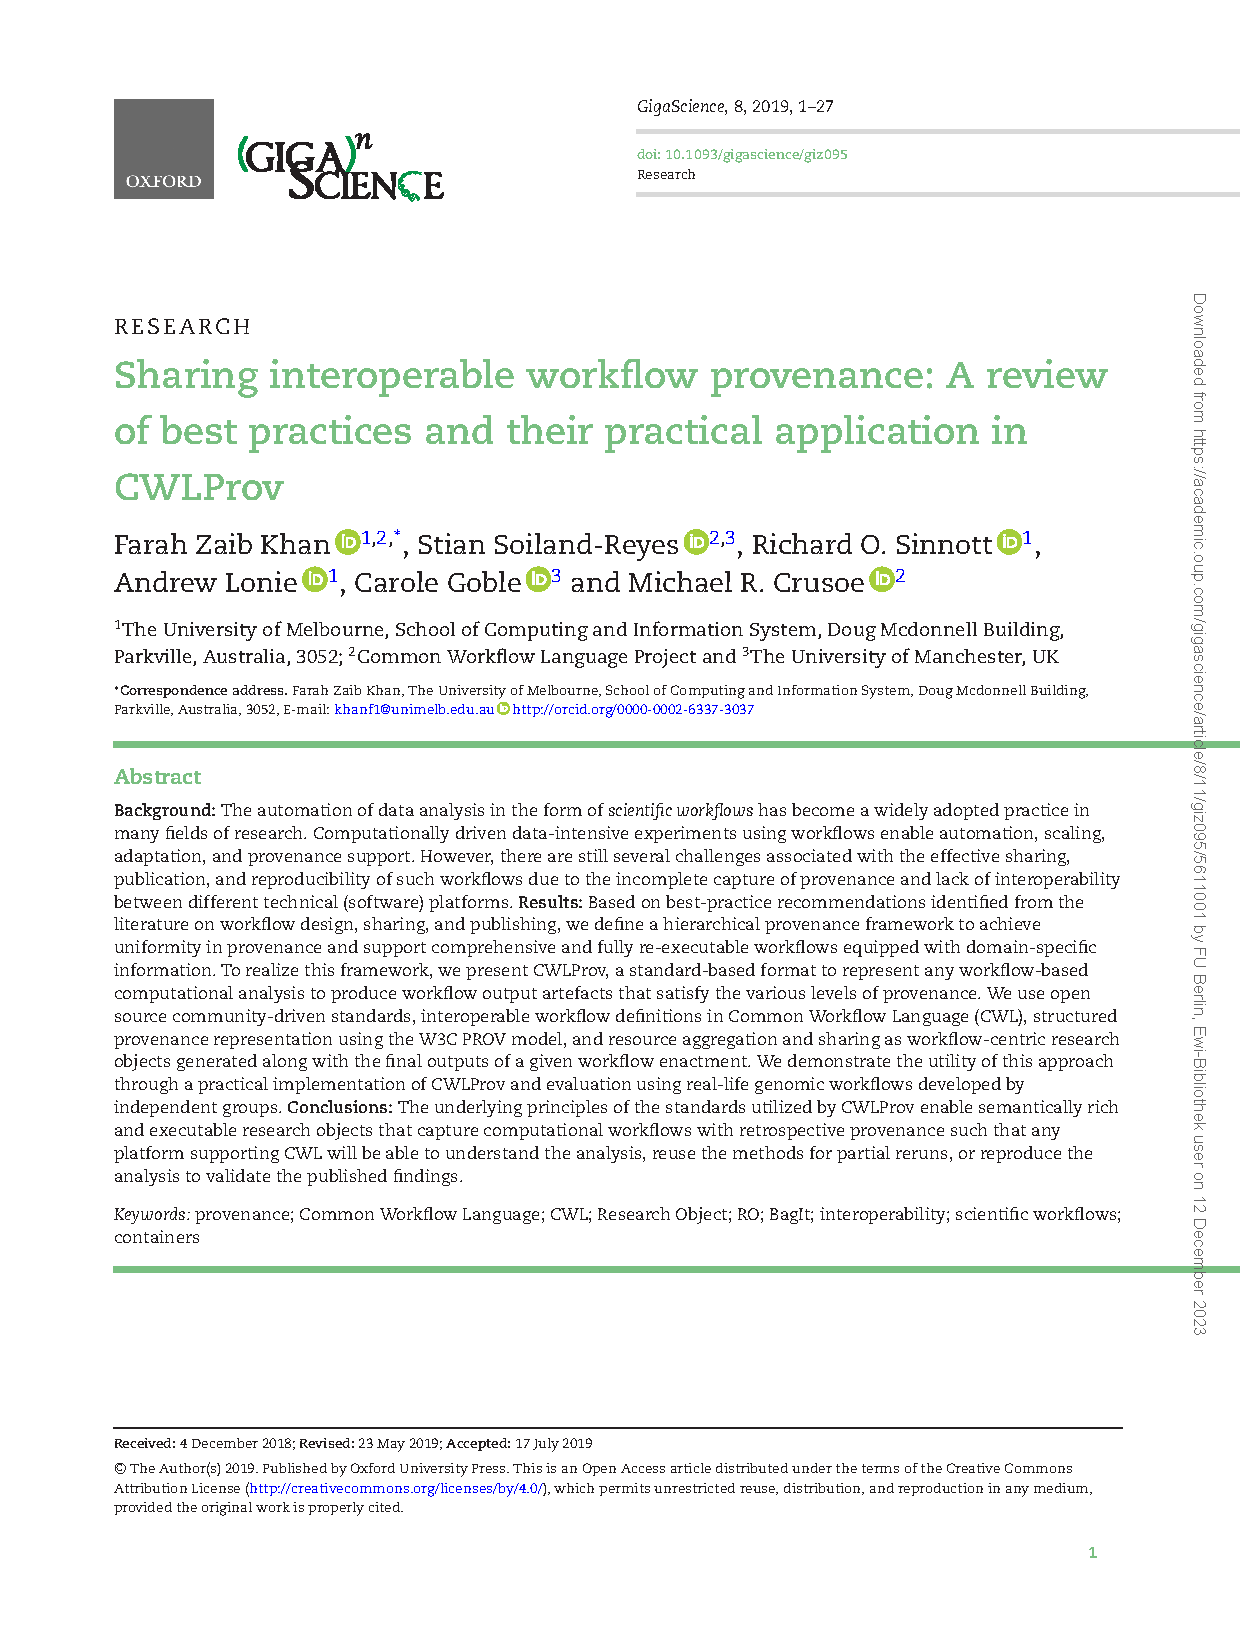
\includepdf[pages=-,addtotoc={2,section,1,Introduction,cwlprov-intro,2,section,1,Background,cwlprov-background,2,subsection,2,Provenance,cwlprov-bg-prov,2,subsection,2,Interoperability,cwlprov-bg-interop,3,subsection,2,Related Work,cwlprov-related,3,subsubsection,3,Workflow software environment capture,cwlprov-related-wfsoftenvcapture,3,subsubsection,3,Data/method {preservation,} {aggregation,} and sharing,cwlprov-related-datamethod,4,subsubsection,3,Provenance capture and standardization,cwlprov-related-provcapture,4,section,1,Levels of Provenance and Resource Sharing,cwlprov-levels-sharing,6,subsection,2,Level 0,cwlprov-level0,7,subsection,2,Level 1,cwlprov-level1,7,subsection,2,Level 2,cwlprov-level2,8,subsection,2,Level 3,cwlprov-level3,8,section,1,CWLProv 0.6.0 and Utilized Standards,cwlprov-0.6.0,9,subsection,2,Applied standards and vocabularies,cwlprov-applied-standards-vocabs,9,subsubsection,3,Common Workflow Language,cwlprov-applied-cwl,9,subsubsection,3,Research Object,cwlprov-applied-ro,10,subsubsection,3,PROV Data Model,cwlprov-applied-prov,11,subsection,2,CWLProv research object,cwlprov-cwlprovrobundle,12,subsection,2,Retrospective provenance profile,cwlprov-retroprov,12,section,1,Practical Realization of CWLProv,cwlprov-practical,14,subsection,2,Achieving recommendations with provenance levels,cwlprov-recs,15,section,1,CWLProv Evaluation with Bioinformatics Workflows,cwlprov-eval,15,subsection,2,Alignment workflow,cwlrpov-eval-alignment,16,subsection,2,Somatic variant calling workflow,cwlprov-eval-somatic,16,subsection,2,Evaluation activity,cwlprov-eval-activity,18,subsection,2,Evaluation results,cwlprov-eval-results,18,subsubsection,3,CWLProv and interoperability,cwlrpov-eval-results-interop,18,subsubsection,3,Evaluating provenance profile,cwlprov-eval-results-provprofile,19,subsubsection,3,Temporal and spatial overhead with provenance,cwlprov-eval-results-overhead,20,subsubsection,3,Output comparison across enactments,cwlprov-eval-results-output-comparison,20,section,1,Discussion and Future Directions,cwlprov-discussion,20,subsection,2,Compute and storage resources,cwlprov-discuss-resources,20,subsection,2,Provenance profile augmented with domain knowledge,cwlprov-discuss-domain,21,subsection,2,Big {-omics} data,cwlprov-discus-bigdata,21,subsection,2,Improving CWLProv efficiency with selective provenance capture,cwlprov-discuss-selective,21,subsection,2,Enforcement of best practices — an open problem,cwlprov-discuss-enforcement,22,section,1,Conclusion,cwlprov-conclusion,22,section,1,Availability of source code and requirements,cwlprov-availability-code,22,section,1,Availability of supporting data and materials,cwlprov-availability-supporting,22,section,1,Abbreviations,cwlprov-abbrevs,22,section,1,Competing interests,cwlprov-competing-interests,23,section,1,Funding,cwlprov-funding,23,section,1,Authors’ contributions,cwlprov-authors-contributions,23,section,1,Acknowledgements,cwlprov-acks,23,section,1,References,cwlprov-refs}]{giz095.pdf}  % CWLProv

\chapter{Recording provenance of workflow runs with RO-Crate}
\label{wrroc}
\bibentry{leo2023recording}

%License

Reproduced here without changes.
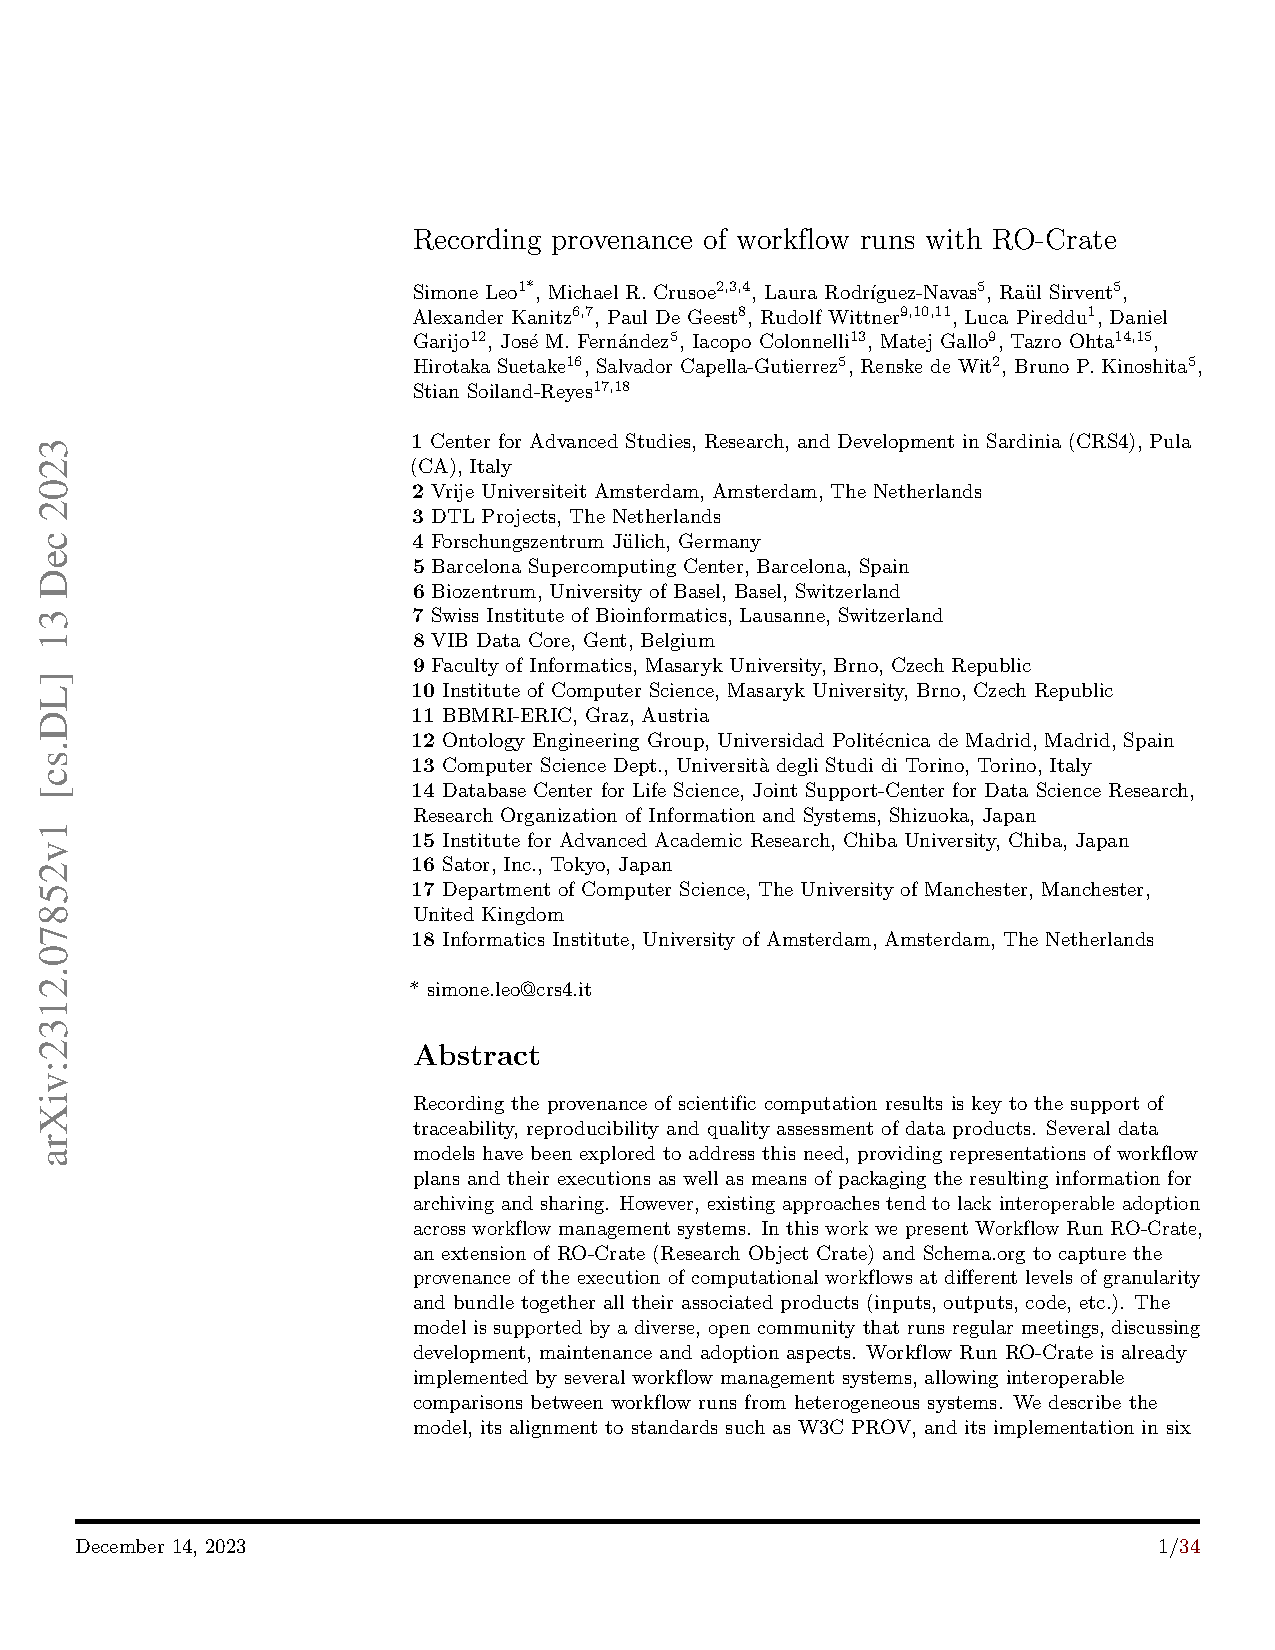
\includepdf[pages=-,addtotoc={2,section,1,Introduction,ro-crate-intro,4,section,1,The Workflow Run RO-Crate profiles,ro-crate-profiles,5,subsection,2,Process Run Crate,ro-crate-process-run,7,subsection,2,Workflow Run Crate,ro-crate-workflow-run,8,subsection,2,Provenance Run Crate,ro-crate-prov-run,10,section,1,Implementations,ro-crate-implementations,11,subsection,2,Runcrate,ro-crate-impl-runcrate,12,subsection,2,Galaxy,ro-crate-impl-galaxy,12,subsection,2,COMPSs,ro-crate-impl-compss,13,subsection,2,StreamFlow,ro-crate-impl-streamflow,14,subsection,2,WfExS-backend,ro-crate-impl-wfexs,15,subsection,2,Sapporo,ro-crate-impl-sapporo,15,subsection,2,Autosubmit,ro-crate-impl-autosubmit,17,subsection,2,Summary of implementations,ro-crate-impl-summary,17,section,1,Exemplary Use Cases,ro-crate-use-cases,17,subsection,2,Provenance Run Crate for Digital Pathology,ro-crate-users-path,20,subsection,2,Process Run Crate and CPM RO-Crate for cancer detection,ro-crate-users-cancer,21,section,1,Discussion,ro-crate-discussion,22,subsection,2,Evaluation of metadata coverage using runcrate convert,ro-crate-discuss-eval,24,subsection,2,Workflow Run RO-Crate and the W3C PROV standard,ro-crate-discussion-w3c,24,subsection,2,Five Safes Workflow Run Crate,ro-crate-discussion-five-safes,25,subsection,2,Biocompute Object RO-Crate,ro-crate-discussion-bco,25,section,1,Conclusion and Future Work,ro-crate-conclusions,26,section,1,Supporting information,ro-crate-supporting-info,26,section,1,Acknowledgments,ro-crate-acks,27,section,1,Author contributions,ro-crate-contribs,28,section,1,References,ro-crate-refs}]{2312.07852.pdf}

\chapter{A Non-Intimidating Approach to Workflow Reproducibility in Bioinformatics: Adding Metadata to Research Objects through the Design and Evaluation of Use-Focused Extensions to CWLProv}
\label{cwlprov-analysis}
%\fullcite{}
%License
Reproduced here without changes.
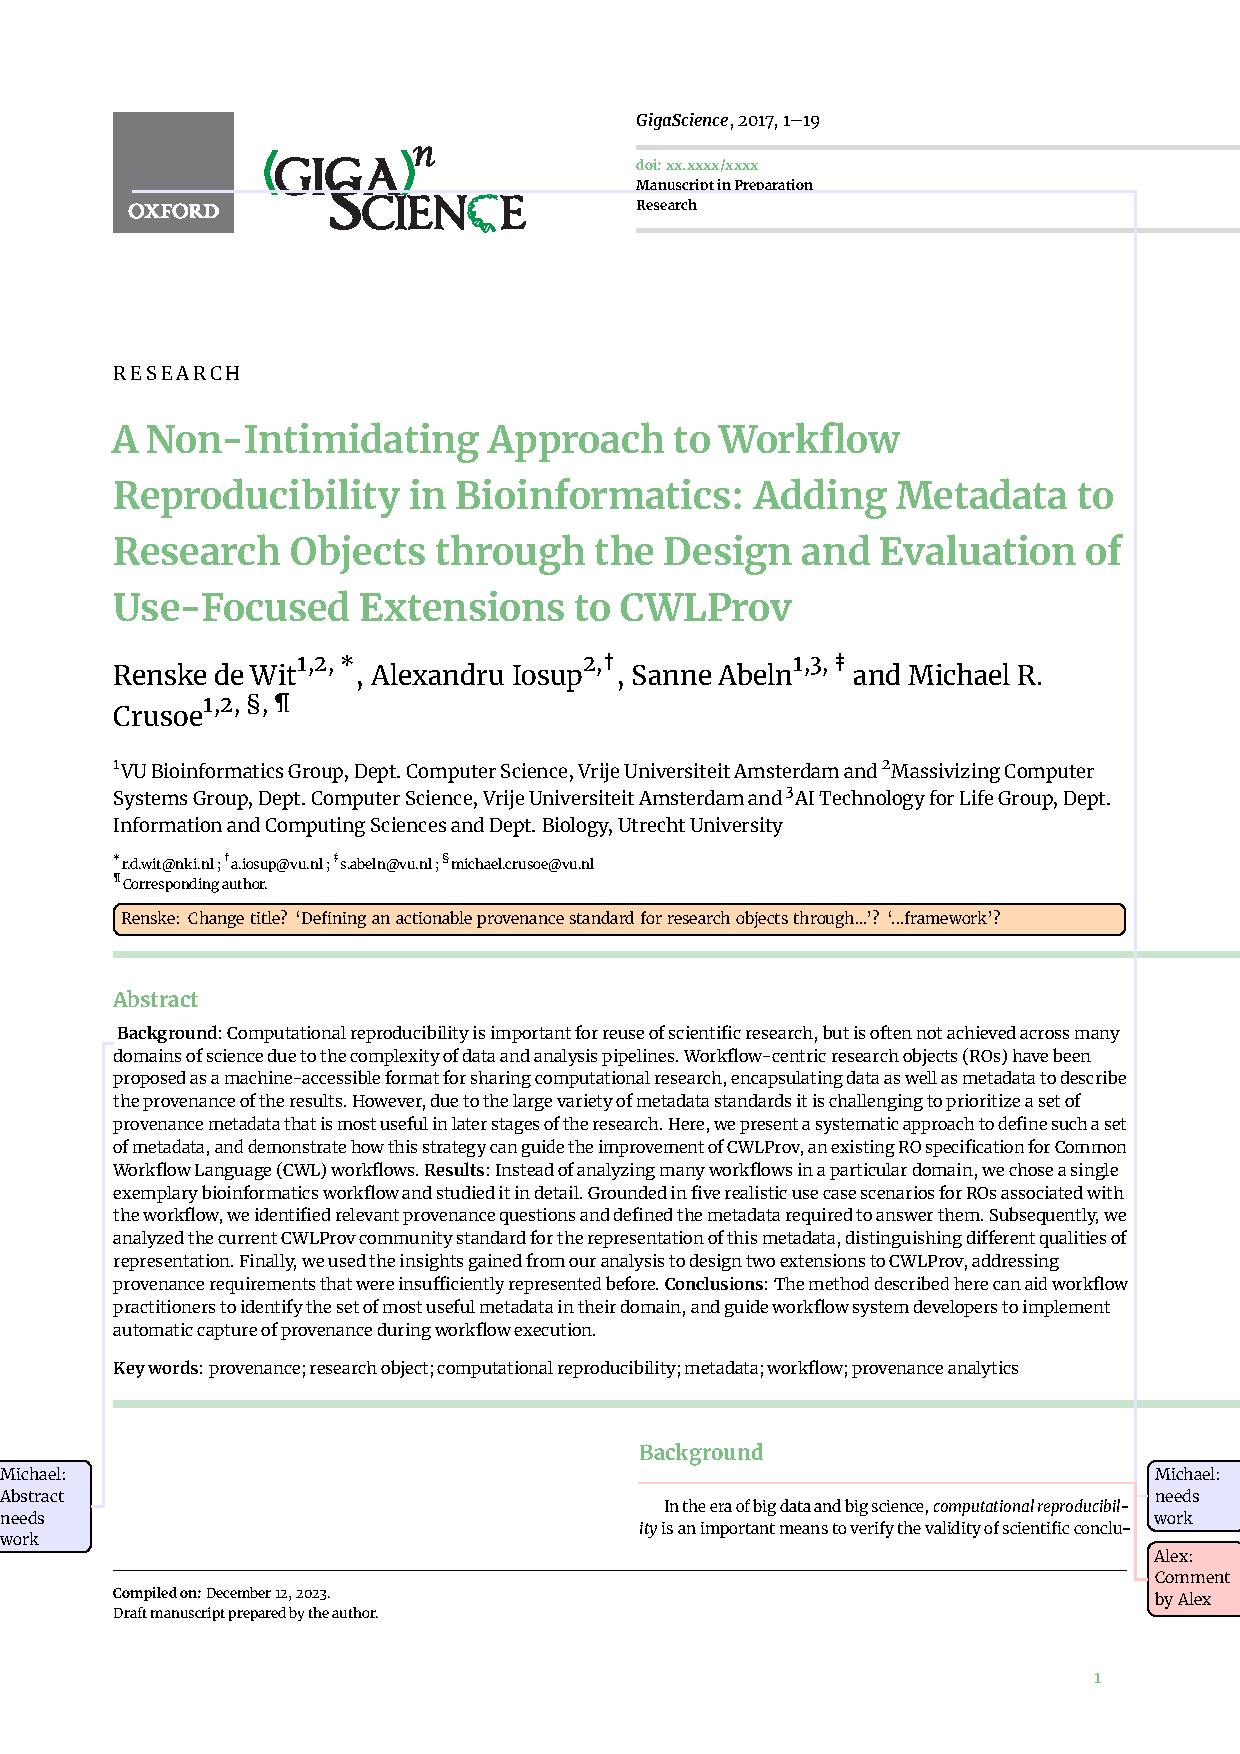
\includepdf[pages=-]{renske-cwlprov-analysis-manuscript.pdf}

\include{conclusion/conclusion}

%% Use letters for the chapter numbers of the appendices.
%\appendix

%\include{appendix-a/appendix-a}

%% Turn off thumb indices for unnumbered chapters.
\thumbfalse

\chapter*{Bibliography}
\addcontentsline{toc}{chapter}{Bibliography}
\setheader{Bibliography}

URLs in this thesis have been archived on Archive.org. Their link target in digital editions refers
to this timestamped version.

\bibliographystyle{unsrt}
% argument is your BibTeX string definitions and bibliography database(s)
\bibliography{dissertation}

%% \chapter*{Glossary}

\glsaddall
\printglossary[type=\acronymtype,title={Glossary}]
\addcontentsline{toc}{chapter}{Glossary}
\setheader{Glossary}

\include{cv/cv}
\include{publications/publications}
%\include{ipa/ipadissertations_2018}

\end{document}

